\documentclass[
	% -- opções da classe memoir --
	12pt,				% tamanho da fonte
	openright,			% capítulos começam em pág ímpar (insere página vazia caso preciso)
	oneside,			% para impressão em frente e verso. Oposto a oneside
	a4paper,			% tamanho do papel.
	% -- opções da classe abntex2 --
	chapter=TITLE,		% títulos de capítulos convertidos em letras maiúsculas
	%section=TITLE,		% títulos de seções convertidos em letras maiúsculas
	%subsection=TITLE,	% títulos de subseções convertidos em letras maiúsculas
	%subsubsection=TITLE,% títulos de subsubseções convertidos em letras maiúsculas
	% -- opções do pacote babel --
	english,			% idioma adicional para hifenização
	french,				% idioma adicional para hifenização
	spanish,			% idioma adicional para hifenização
	brazil				% o último idioma é o principal do documento
	]{abntex2}
% ---
% Pacotes básicos 
% ---
\usepackage{lmodern}			% Usa a fonte Latin Modern
\usepackage{mathptmx}			% Usa a fonte Times New Roman
\usepackage[T1]{fontenc}		% Selecao de codigos de fonte.
\usepackage[utf8]{inputenc}		% Codificacao do documento (conversão automática dos acentos)
\usepackage{lastpage}			% Usado pela Ficha catalográfica
\usepackage{indentfirst}		% Indenta o primeiro parágrafo de cada seção.
\usepackage{color}				% Controle das cores
\usepackage{graphicx}			% Inclusão de gráficos
\usepackage{subcaption}				% Inclusão de gráficos lado a lado
\usepackage{microtype} 			% para melhorias de justificação
\usepackage{tabularx,ragged2e}	% Para inserir tabelas
\usepackage{multirow}			% Para mesclar células
\usepackage[dvipsnames,table,xcdraw]{xcolor}		% Permite adicionar cores nas linhas de tabelas
\usepackage{fancyvrb}			% Permite adicionar arquivos de texto
\usepackage[portuguese, ruled, linesnumbered]{algorithm2e} % Uso de algoritmos
\usepackage{amsfonts}			% Permite usar notação de conjuntos
\usepackage{amsmath}			% Permite citar equações
\usepackage{amsthm}				% Permite criar teoremas e experimentos
\usepackage[font={bf, small}, labelsep=endash, labelfont=bf]{caption}	% Faz legenda de figuras ficarem em negrito
\usepackage{cancel}				% Permite fazer expressão tendendo a zero
\usepackage{epstopdf}			% Converte eps para pdf
\usepackage[final]{pdfpages}
\usepackage{hyperref}
\usepackage{fancybox}

\bibliographystyle{plain}

\newcolumntype{L}{>{\RaggedRight\arraybackslash}X}
% ---
% ---
% Pacotes adicionais, usados apenas no âmbito do Modelo Canônico do abnteX2
% ---
\usepackage{lipsum}				% para geração de dummy text
% ---
% ---
% Pacotes de citações
% ---
%\usepackage[brazilian,hyperpageref]{backref}	 % Paginas com as citações na bibl
\usepackage[alf, abnt-emphasize=bf]{abntex2cite}	% Citações padrão ABNT
% ---
% Customizações para o layout da UFPA
% ---
\usepackage{modelo-ufpa/ufpa}
% Muda o título de lista de ilustrações para lista de figuras
\addto\captionsbrazil{%
  \renewcommand{\listfigurename}%
    {Lista de Ilustrações}%
	\renewcommand{\listtablename}%
    {Lista de Tabelas}%
}
% Permite utilizar figuras sem precisar colocar o caminho absoluto
\graphicspath{{imagens/}}
% Define o ambiente de experimentos
\theoremstyle{definition}
\newtheorem{experimento}{Experimento}[section]
\newcommand{\experimentoautorefname}{Experimento}


% --------------------------------------------------------------
% Informações do TRABALHO
% --------------------------------------------------------------
\universidade{UNIVERSIDADE FEDERAL DO PARÁ}
\instituto{INSTITUTO DE TECNOLOGIA}
\faculdade{FACULDADE DE COMPUTAÇÃO E TELECOMUNICAÇÕES}
%\curso{CURSO DE BACHARELADO EM SISTEMAS DE INFORMAÇÃO}
\titulo{RELATÓRIO DE SISTEMAS OPERACIONAIS}
\autor{
%\begin{tabular}{l l}
    DAVID PINHEIRO DE SOUSA - 202207040045 \\
    JOAO VICTOR SANTOS BRITO FERREIRA - 202207040028 \\
    JOEL TAVARES MIRANDA - 202206840054 \\
    KAUAN MIRANDA TAVARES - 202206840033 \\
    MARCO ANTONIO DO ESPIRITO SANTO MAUES JUNIOR - 202206840038 \\
%\end{tabular}
}
\local{Belém}
\data{2023}
\orientador{Prof. Dr. Diego Lisboa Cardoso}
\tipotrabalho{Monografia}

% o nome da instituição e a área de concentração 
\preambulo{Relatório do trabalho 1 de Sistemas Operacionais.}
%\sobrenome{Sobrenome}
%\nome{Nome}
%\palavraschave
%\datadadefesa{Data da Defesa: 09 de Março de 2017}%07 de Dezembro de 2016}
\conceito{Conceito: Excelente}
\faculdadedoorientador{Faculdade de  - UFPA}
\primeiromembrodabanca{Prof. Dr. Nome Sobrenome}
\faculdadedoprimeiromembrodabanca{Faculdade de  - UFPA}
\segundomembrodabanca{Prof. Dra. Nome Sobrenome}
\faculdadedosegundomembrodabanca{Faculdade de  - UFPA}
% -------------------------------------------------------------------------
% ---
% Configurações de aparência do PDF final
% alterando o aspecto da cor azul
\definecolor{blue}{RGB}{41,5,195}
% informações do PDF
\makeatletter
\hypersetup{
     	%pagebackref=true,
		pdftitle={\imprimirtitulo}, 
		pdfauthor={\imprimirautor},
    	pdfsubject={\imprimirpreambulo},
	    pdfcreator={LaTeX with abnTeX2},
		pdfkeywords={\imprimirpalavraschave}, 
		colorlinks=true,       		% false: boxed links; true: colored links
    	linkcolor=black,          	% color of internal links
    	citecolor=black,        		% color of links to bibliography
    	filecolor=magenta,      		% color of file links
		urlcolor=blue,
		bookmarksdepth=4,
        breaklinks=true
}
\makeatother
% --- 
% Espaçamentos entre linhas e parágrafos 
% --- 
% O tamanho do parágrafo é dado por:
\setlength{\parindent}{1.3cm}
% Controle do espaçamento entre um parágrafo e outro:
\setlength{\parskip}{0.2cm}  % tente também \onelineskip
% compila o indice
% ---
\makeindex
% ---

% -------------------------------------------------------------------------
% ---------------------------INICIO DO DOCUMENTO---------------------------
% -------------------------------------------------------------------------
\begin{document}
% Seleciona o idioma do documento (conforme pacotes do babel)
\selectlanguage{brazil}
% Retira espaço extra obsoleto entre as frases.
\frenchspacing 
% ----------------------------------------------------------
% ELEMENTOS PRÉ-TEXTUAIS
% ----------------------------------------------------------
% \pretextual

% ---
% Capa
% ---
\imprimircapa
% ---

% ---
% Folha de rosto

\imprimirfolhaderosto

\newpage

\setlength{\absparsep}{18pt} % ajusta o espaçamento dos parágrafos do resumo

\pdfbookmark[0]{\contentsname}{toc}
\tableofcontents*
\cleardoublepage
% ---
% ---------------------------------------------------------
% ELEMENTOS TEXTUAIS
% ----------------------------------------------------------
\textual

% ----------------------------------------------------------
% Introdução
% ----------------------------------------------------------

\chapter{Introdução}

A literatura de sistemas operacionais está cheia de problemas interessantes que foram amplamente discutidos e analisados usando variados métodos de sincronização \cite{tanenbaum2010sistemas}. Os problemas clássicos de sistemas operacionais são exemplos de problemas de coordenação de processos, comumente abordados por autores e em sala de aula. Muitos desses problemas são didaticamente importantes para a compreensão do tema IPC (Interprocess Communication), onde situações adversas e/ou indesejadas durante a execução de processos e threads devem ser solucionadas para o bem da concorrência entre tarefas e sistemas multiprogramáveis. Nesse contexto, o presente trabalho busca analisar soluções de alguns desses problemas clássicos.

\chapter{Objetivos}

O objetivo deste trabalho é analisar soluções dos seguintes problemas clássicos da literatura de sistemas operacionais:

\begin{itemize}
	\item \textbf{O Problema do Leitores x Escritores}
        %\ovalbox{sys\_read}
	\item \textbf{O Jantar dos Filósofos}
	\item \textbf{O Problema do Produtor x Consumidor}
	\item \textbf{O Problema do Barbeiro Dorminhoco}
  \end{itemize}
  

\chapter{O Problema do Leitores x Escritores}

\section{Descrição do problema}
O problema dos Leitores x Escritores é um conhecido paradigma da Programação Concorrente. Este problema parte do princípio da existência de vários processos ou threads de duas naturezas distintas: leitores e escritores. Todos compartilham uma zona de memória comum, no qual escritores modificam um dado, e leitores leem esse dado. O problema se dá pela necessidade de sincronização entre essas duas naturezas para que não haja distúrbio causado por possíveis condições de corrida. 

Sendo assim, a ideia é coordenar tais tarefas de modo que a medida que leitores chegam, podem ler à vontade, contanto que haja pelo menos um leitor agindo na zona compartilhada. O que não pode acontecer é que mais de um escritor entre em ação, não importa quantas ou de que tipo as tarefas fora da região crítica desejarem utilizá-la.

A \textbf{Figura~\ref{fig:ex_leitor_escritor}} abaixo exemplifica uma situação onde um buffer M é comparilhado por escriores (e) e leitores (l).

\begin{figure}[h]
    \centering
    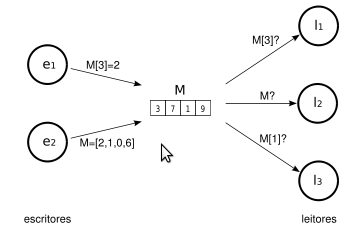
\includegraphics[width=0.7\textwidth]{imagens/leitor_escritor.jpg}
    \caption{Leitores e escritores: Exemplo ilustrativo}
    \label{fig:ex_leitor_escritor}
\end{figure}

Portanto, para desenvolver uma solução, é preciso atender às seguintes condições:

\begin{itemize}
    \item Para um leitor acessar a zona compartilhada, basta certificar-se que haja pelo menos um outro leitor ativo na mesma;
    \item Um escritor, para ter acesso à zona compartilhada, precisa garantir acesso exclusivo;
    \item Tarefas de tipos distintos não podem ter acesso simultâneo à zona compartilhada.
\end{itemize}

\section{Implementação em C}

\subsection{Contexto}

Existe certa quantidade de tarefas Leitores e Escritores que compartilham uma base de dados que guarda uma variável contador. Para evitar a condição de corrida, é preciso coordenar o acesso à base de dados para a leitura e escrita da variável contador.

\subsection{Proposta} 

A solução proposta, implementada em C, faz uso de semáforos para controlar o acesso à zona de memória compartilhada (base de dados) e a uma variável que indica a quantidade de leitores ativos no momento. Assim, para acessarem a base de dados, leitores e escritores devem, primeiramente, solicitar acesso aos semáforos, garantindo a exclusão mútua, quando necessária.

\subsection{Código}

O código-fonte em C utiliza as seguintes bibliotecas:
\begin{itemize}
    \item \textbf{\ovalbox{pthread.h}}: Para criação e gerenciamento de threads e mutexes;
    \item \textbf{\ovalbox{semaphore.h}}: Para implementação de semáforos;
    \item \textbf{\ovalbox{stdio.h}} e \textbf{\ovalbox{stdlib.h}}: Bibliotecas-padrão de entrada e saída;
    \item \textbf{\ovalbox{unistd.h}}: Para o uso de funções como \ovalbox{sleep()};
    \item \textbf{\ovalbox{locale.h}}: Para impressão de saída em língua portuguesa.
\end{itemize}

O primeiro trecho de código é dado a seguir:

\begin{verbatim}
// DEFINIÇÃO DE MACROS:
#define LEITORES 10 // Número de leitores
#define ESCRITORES 5 // Número de escritores

// SEMÁFOROS:
pthread_mutex_t db; // 'db': Garante acesso à base de dados.
pthread_mutex_t mutex; // 'mutex': Garante acesso à variável 'leitor_lendo'.

int leitor_lendo, // Representa o número de leitores ativos no momento.
cnt = 0; // O contador 'cnt' representa o dado compartilhado.

// FUNÇÕES DE AÇÃO:
void ler_base_de_dados(void*ln); // Leitura abstrata da base de dados
void usar_banco_de_dados(void*ln); // Uso do dado lido
void pensando_nos_dados(void* en); // Escritores "definem" o dado
void escrever_no_banco_de_dados(void* en); // Escritores modificam o dado
\end{verbatim}

Os macros \ovalbox{LEITORES} e \ovalbox{ESCRITORES} definem o número de leitores e escritores, respectivamente. Os semáforos mutex \ovalbox{db} e \ovalbox{mutex} são utilizados para garatir acesso exclusivo, por essa ordem, à base de dados e ao contador de leitores, \ovalbox{leitores\_lendo}. Além desse, outro contador, \ovalbox{cnt} é usado para representar o dado que sofre escrita e leitura. Tendo isso definido, logo abaixo encontram-se os protótipos das funções de ação dos leitores e escritores:

\begin{itemize}
    \item \textbf{\ovalbox{ler\_base\_de\_dados()}}: Função de leitura da base de dados;
    \item \textbf{\ovalbox{usar\_banco\_de\_dados()}}: Função de "uso" do dado lido;
    \item \textbf{\ovalbox{pensando\_nos\_dados()}}: Função de produção do dado a ser escrito;
    \item \textbf{\ovalbox{escrever\_no\_banco\_de\_dados()}}: Função de escrita na base de dados.
\end{itemize}

A função característica dos leitores é dada a seguir:

\begin{verbatim}
// FUNÇÃO 'leitor()':
void leitor(void* ln){
    while(1){
        pthread_mutex_lock(&mutex); // Acesso à variável 'leitor_lendo'
        leitor_lendo++;

        if(leitor_lendo == 1) 
            pthread_mutex_lock(&db); // Acesso à base de dados
        pthread_mutex_unlock(&mutex);   // Libera 'leitor_lendo'

        ler_base_de_dados(ln); // Leitura do dado compartilhado
        pthread_mutex_lock(&mutex); // Acesso à variável 'leitor_lendo'
        leitor_lendo--; 

        if(leitor_lendo == 0) 
            pthread_mutex_unlock(&db); // Libera o acesso à base de dados
        pthread_mutex_unlock(&mutex); // Libera 'leitor_lendo'
        
        usar_banco_de_dados(ln); // Usa o dado
    }
}
\end{verbatim}

Na função \ovalbox{leitor(void*ln)}, o argumento \ovalbox{void* ln} identifica o leitor. Dentro do loop infinito, \ovalbox{while(1)}, ocorre o seguinte procedimento:

\begin{enumerate}
    \item Solicita acesso exclusivo ao contador \ovalbox{leitor\_lendo}. Tendo acesso, prossegue, senão espera;
    \item Incrementa o contador \ovalbox{leitor\_lendo};
    \item Se o leitor em questão for o primeiro, solicita acesso exclusivo à base de dados para os grupo leitores pelo semáforo \ovalbox{db}. Tendo acesso, prossegue, senão espera. Se não for o primeiro, prossegue;
    \item Libera o contador \ovalbox{leitor\_lendo};
    \item Lê o dado compartilhado pela função \ovalbox{ler\_base\_de\_dados};
    \item Solicita acesso exclusivo ao contador \ovalbox{leitor\_lendo}. Tendo acesso, prossegue, senão espera;
    \item Decrementa o contador \ovalbox{leitor\_lendo};
    \item Caso o leitor em questão for o último, libera o semáforo \ovalbox{db}, se não, prossegue;
    \item Libera o contador \ovalbox{leitor\_lendo};
    \item Utiliza o dado lido, pela função \ovalbox{usar\_banco\_de\_dados()}.
    \item Retorna ao passo 1.
\end{enumerate}

Logo após, segue a função característica dos escritores:

\begin{verbatim}
// FUNÇÃO 'escritor()':    
void escritor(void* en){
    
    while(1){
        pensando_nos_dados(en); // Passa um tempo na função
        pthread_mutex_lock(&db); // Acesso à base de dados
        escrever_no_banco_de_dados(en); // Escrita na base de dados

        pthread_mutex_unlock(&db); // Libera a base de dados
    }
}
\end{verbatim}

Na função \ovalbox{escritor(void*en)}, o argumento \ovalbox{void*en} serve como identificador do escritor em questão. Ao que segue no loop infinito \ovalbox{while(1)}, temos o procedimento:

\begin{enumerate}
    \item "Pensa", isto é, "produz" o dado que será escrito, pela função \ovalbox{pensando\_nos\_dados()};
    \item Solicita acesso exclusivo à base de dados, pelo semáforo \ovalbox{db}. Tendo acesso, prossegue, senão espera;
    \item Modifica o dado compartilhado \ovalbox{cnt}, pela função \ovalbox{escrever\_no\_banco\_de\_dados()};
    \item Libera o semáforo \ovalbox{db};
    \item Retorna ao passo 1.
    
\end{enumerate}

A demais funções são descritas a seguir:

\begin{verbatim}
// FUNÇÃO 'ler_base_de_dados()':
void ler_base_de_dados(void*ln){
    setlocale(LC_ALL, "Portuguese");
        int tempo_de_leitura;
        tempo_de_leitura = rand() % 5;
        printf("\033[0;32m");
        printf("Leitor %d LENDO %d do banco de dados. Total de %d 
        leitores LENDO agora.\n", *((int*)ln), cnt,leitor_lendo);
        sleep(tempo_de_leitura);
}
// FUNÇÃO 'usar_banco_de_dados':
void usar_banco_de_dados(void*ln){
    setlocale(LC_ALL, "Portuguese");
        int tempo_de_uso;
        tempo_de_uso = rand() % 15;
        printf("\033[0;34m");
        printf("A partir do leitor %d, usuário está utilizando o contador %d 
        adquirido no banco de dados.\n", *((int*)ln), cnt);
        sleep(tempo_de_uso);
}
/*FUNÇÃO 'pensando_nos_dados':
void pensando_nos_dados(void*en){
    setlocale(LC_ALL, "Portuguese");
        int tempo_para_pensar;
        tempo_para_pensar = rand() % 10;
        printf("\033[0;34m");
        printf("Escritor %d PENSANDO no que irá escrever.\n", *((int*)en));
        sleep(tempo_para_pensar);
}
/*FUNÇÃO 'escrever_no_banco_de_dados':
void escrever_no_banco_de_dados(void* en){
    setlocale(LC_ALL, "Portuguese");
        int tempo_de_escrita;
        tempo_de_escrita = rand() % 10;
        cnt++;
        printf("\033[0;31m");
        printf("Escritor %d ESCREVENDO no banco de dados. 
                Contador em %d\n", *((int*)en), cnt);
        sleep(tempo_de_escrita);
}
\end{verbatim}

Cada uma dela procede a seguinte lógica: Define-se um tempo aleatório entre 0 a 15 segundos, definindo o tempo de suspensão da execução da thread em questão, após imprimir na tela o resultado da ação que compete à função. Essa ação pode ser de leitura, pela função \ovalbox{ler\_base\_de\_dados()}, de escrita, pela função \ovalbox{escrever\_no\_banco\_de\_dados()}, de uso de dados, pela função \ovalbox{usar\_banco\_de\_dados} ou de produção de dados, pela função \ovalbox{pensando\_nos\_dados}.

A função principal \ovalbox{main} é responsável pela inicialização dos semáforos, criação e manutenção das threads escritores e leitores, e fluxo principal do programa, como mostra o trecho de código a seguir:

\begin{verbatim}
int main(){
    // THREADS: 'escritores' e 'leitores'
    pthread_t escritores[ESCRITORES], leitores[LEITORES];
    int i;
    // INICIALIZAÇÃO: semáforos 'db' e 'mutex'
    pthread_mutex_init(&db, NULL);
    pthread_mutex_init(&mutex, NULL);

    // CRIAÇÃO DAS THREADS DE ESCRITORES
    for(i=0; i<ESCRITORES; i++){
        int* escritor_id = malloc(sizeof(int));
        *escritor_id = i+1; // ID relativa da thread 
        pthread_create(&escritores[i], NULL, (void*) escritor, 
                                            (void*) escritor_id);
    }
    // CRIAÇÃO DAS THREADS DE LEITORES
    for(i=0; i<LEITORES; i++){
        int* leitor_id = malloc(sizeof(int));
        *leitor_id = i+1; // ID relativa da thread
        pthread_create(&leitores[i], NULL, (void*) leitor, (void*) leitor_id);
    }
    // SINCRONIZAÇÃO DAS THREADS DE ECRITORES
    for(i=0; i<ESCRITORES; i++){
        pthread_join(escritores[i], NULL);
    }
    // SINCRONIZAÇÃO DAS THREADS DE LEITORES
    for(i=0; i<LEITORES; i++){
        pthread_join(leitores[i], NULL);
    }
    return 0;
}
\end{verbatim}

O código declara 10 leitores, \ovalbox{leitores[LEITORES]} e 5 escritores \ovalbox{escritores[ESCRITORES]} do tipo \ovalbox{pthread\_t} - quantidades de acordo com os macros definidos no princípio do código -, e as inicializa usando a função \ovalbox{pthread\_create}, passando a função respectiva, \ovalbox{leitor()} ou \ovalbox{escritor()}, e um identificador \ovalbox{id}. Cada thread de leitor e escritor tem um identificador relativo \ovalbox{leitor\_id} ou \ovalbox{escritor\_id}, utilizados para facilitar a visualização da saída. 

O código completo está disponibilizado, juntamente com as instruções, no \href{https://github.com/jvictorferreira3301/Sistemas_Operacionais}{nosso repositório da disciplina}.

Após a inicialização, as threads são sincronizadas por meio da função \ovalbox{pthread\_join}, garantindo que elas se comportem conforme o esperado e evitando problemas comuns de concorrência, como condições de corrida e vazamentos de recursos. Na próxima seção, é possível ver o resultado da execução do código proposto para a solução do problema Leitor x Escritor.

\subsection{Execução}

A seguir, a \textbf{Figura~\ref{fig:1}} mostra uma captura de saída durante a execução do código \ovalbox{leitor\_escritor.c}.

\begin{figure}[h]
    \centering
    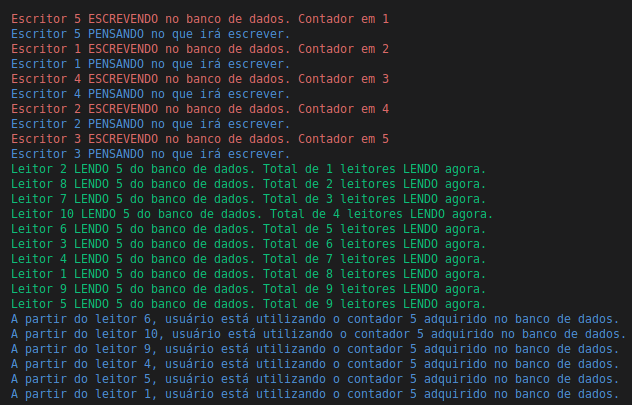
\includegraphics[width=1.0\textwidth]{imagens/out_leitor_escritor.png}
	\caption{Saída no terminal do leitor\_escritor.c}
	\label{fig:1}
\end{figure}

Por meio da \textbf{Figura~\ref{fig:1}}, pode ser observado a concorrência entre os escritores 5, 1, 4, 2 e 3, que modificam, exclusivamente, o contador \ovalbox{cnt}, imprimindo na tela seu valor. Logo após todos os escritores terminarem seus trabalhos de escrita, um grupo de leitores tem acesso liberado à base de dados, adquirindo a última última modificação do contador \ovalbox{cnt}. Observe que, conforme vão chegando novos leitores, o tamanho do grupo aumenta, e o acesso ao contador \ovalbox{cnt} é simultâneo entre os leitores. Contudo, a proposta atende às condições estabelecidas para a solução do problema.

\subsection{Análise}
\subsubsection{Da solução implementada}

A solução implementada consegue atender aos requisitos para o funcionamento correto das atividades dos leitores e escritores. O uso do semáforo mutex \ovalbox{db} é crucial para restringir o acesso de threads de natureza diferentes à base de dados que contém o dado compartilhado \ovalbox{cnt}. 

Outro ponto importante é o uso controlado, por meio do mutex \ovalbox{mutex}, da variável \ovalbox{leitor\_lendo}, que ajuda no controle do número de leitores ativos e permite que um leitor não impessa um novo leitor que chega na fila de executar simultaneamente, até que um escritor solicite acesso.

Assim, a estrutura geral da solução permite que threads de leitura e escrita concorram de forma saudável ao recurso compartilhado.

\subsubsection{De possíveis melhorias}

Analisando o código atual, é possível citar melhorias que podem ser implementadas:
\begin{enumerate}
    \item A função \ovalbox{pensando\_nos\_dados} está sendo usada para suspender a execução por um intervalo de tempo, mas pode ser modificada para que um item aleatório seja criado, gerando um dado que pode ser retornado e usado para modificar a base de dados.
\end{enumerate}
\newpage
\section{Capturas da IDE mostrando o código}

Nesta seção serão apresentadas capturas da tela da IDE mostrando os códigos apresentados acima, que se encontram, também disponíveis no
\href{https://github.com/jvictorferreira3301/Sistemas_Operacionais}{nosso repositório da disciplina}.
Por conta do código em C ser muito extenso optamos por apresentar o mesmo em partes separadas. O código completo pode ser acessado no repositório.

\begin{figure}[h]
    \centering
    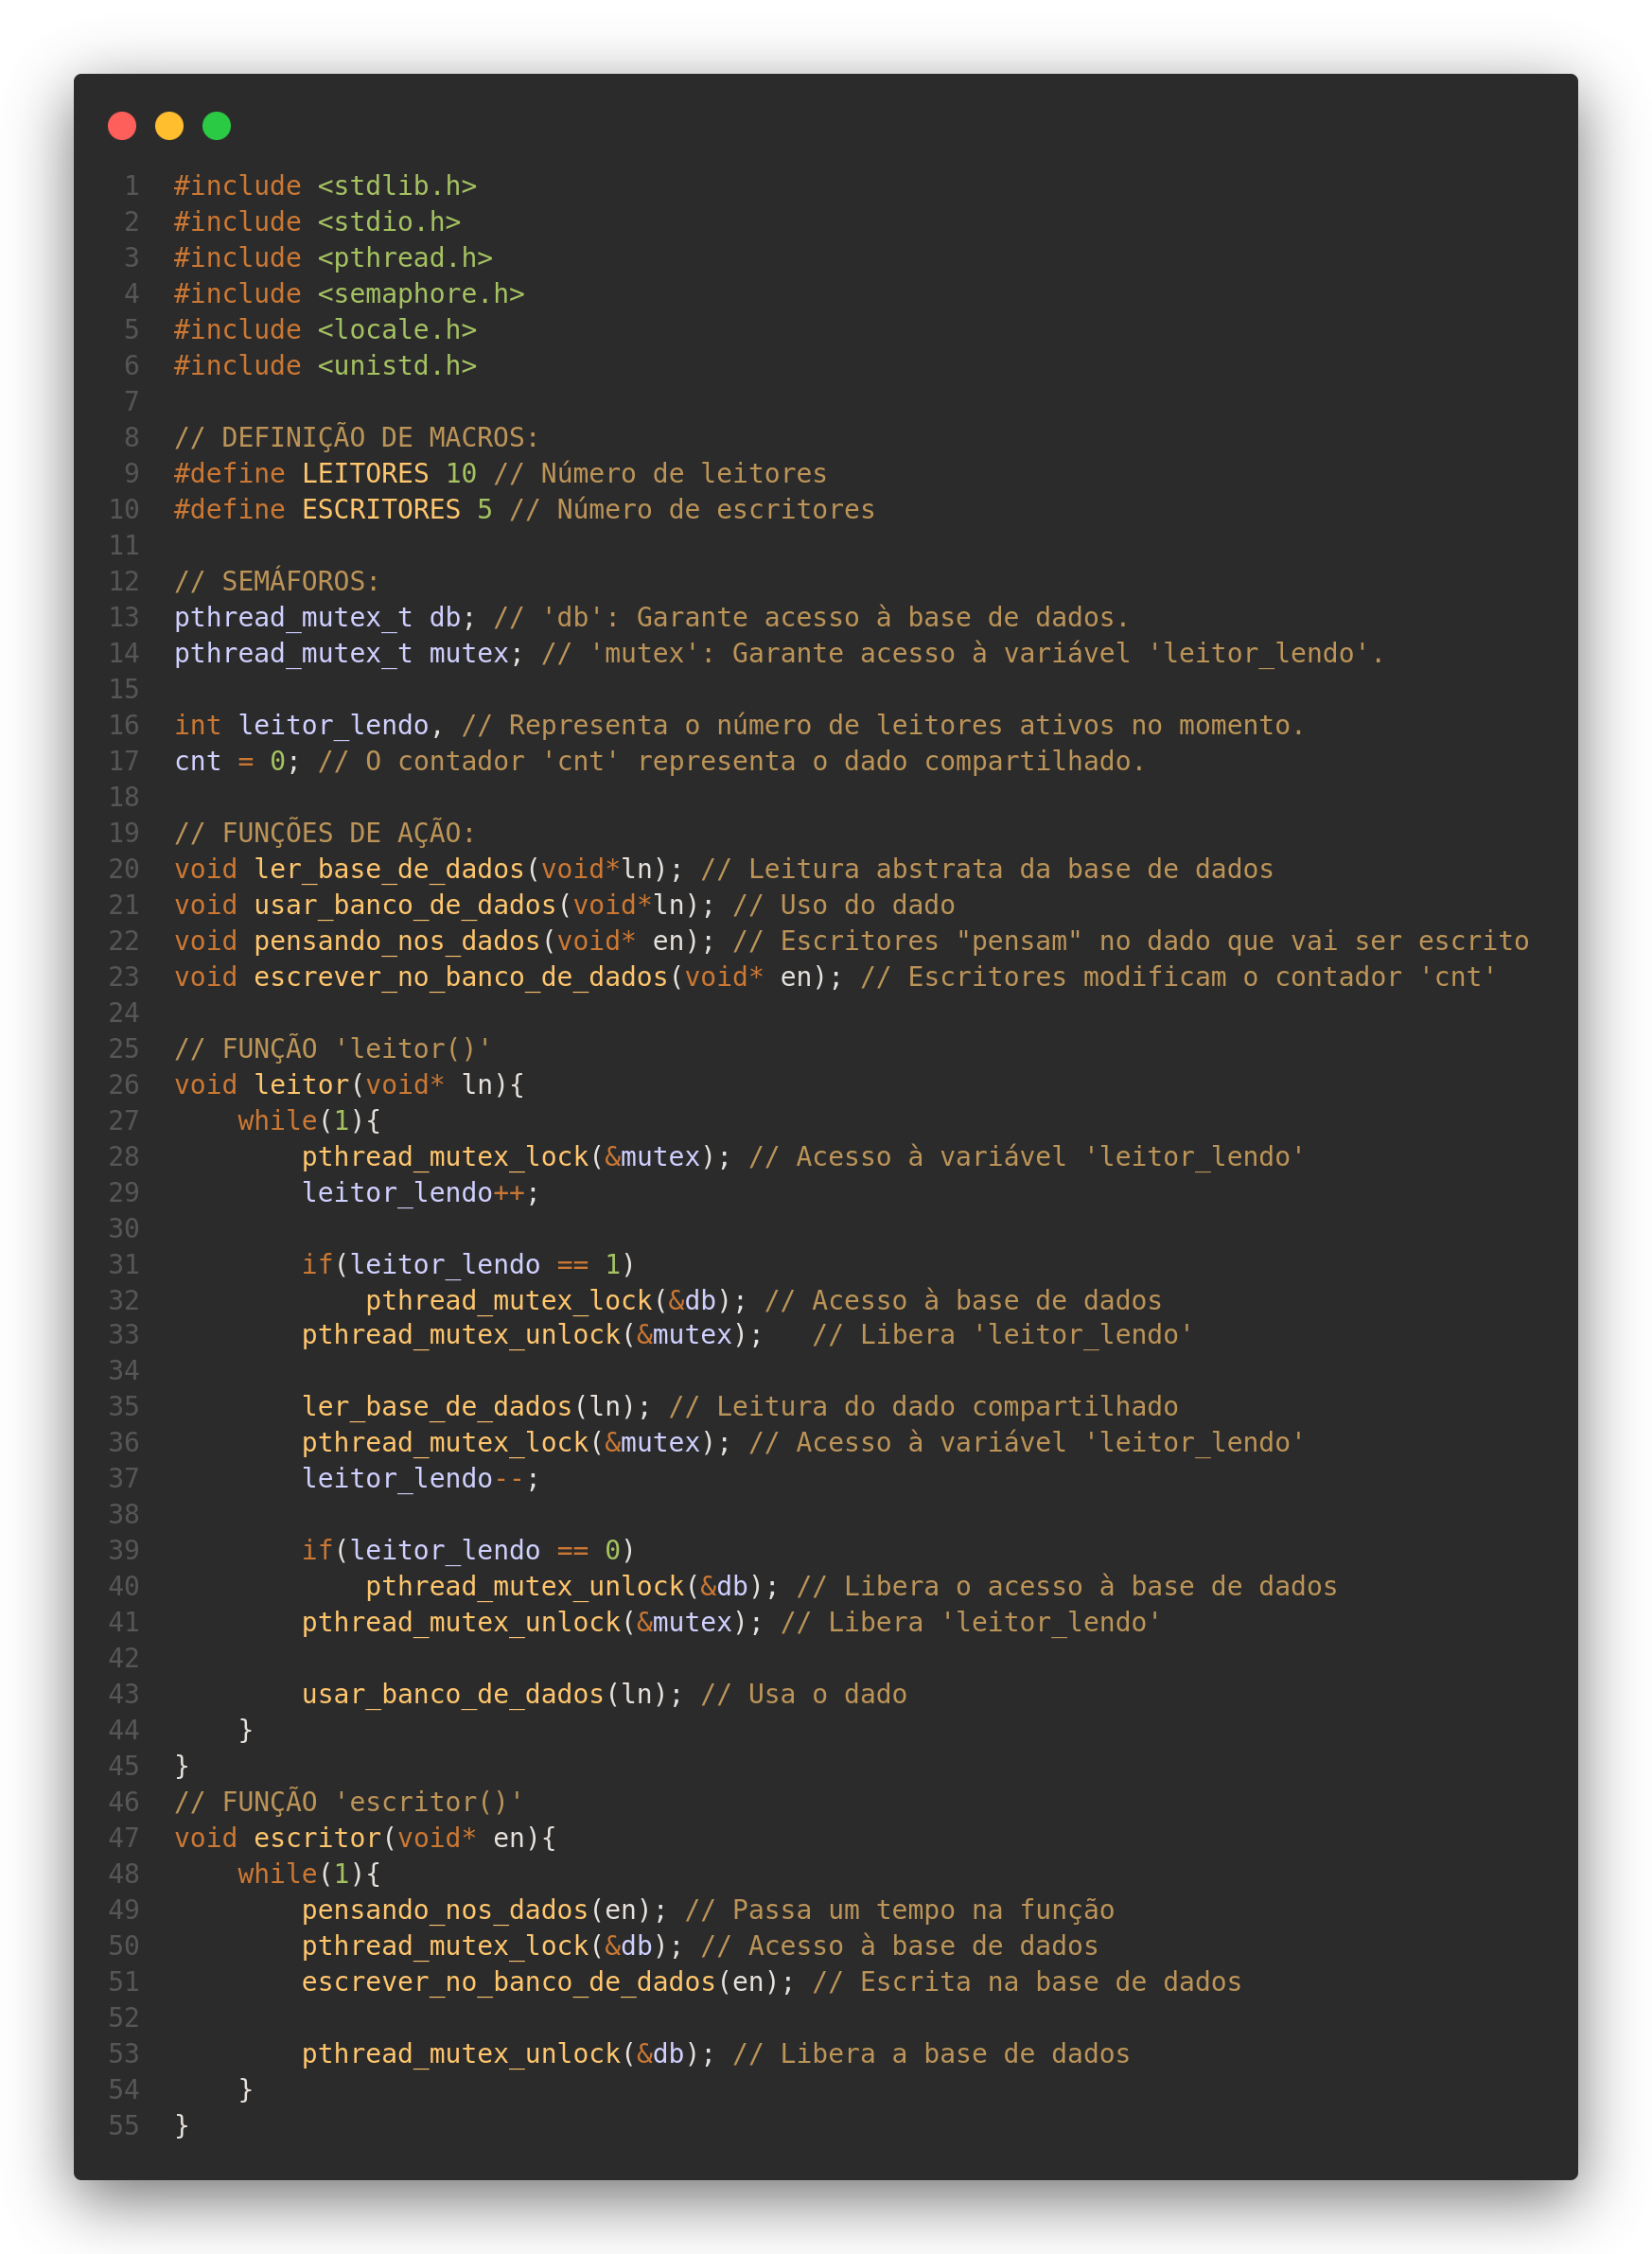
\includegraphics[width=0.9\textwidth]{imagens/leitor_escritor_1.png}
    \caption{Leitor x Escritor: Código em C - Parte I}
    \label{fig:2}
\end{figure}

\begin{figure}[h]
    \centering
    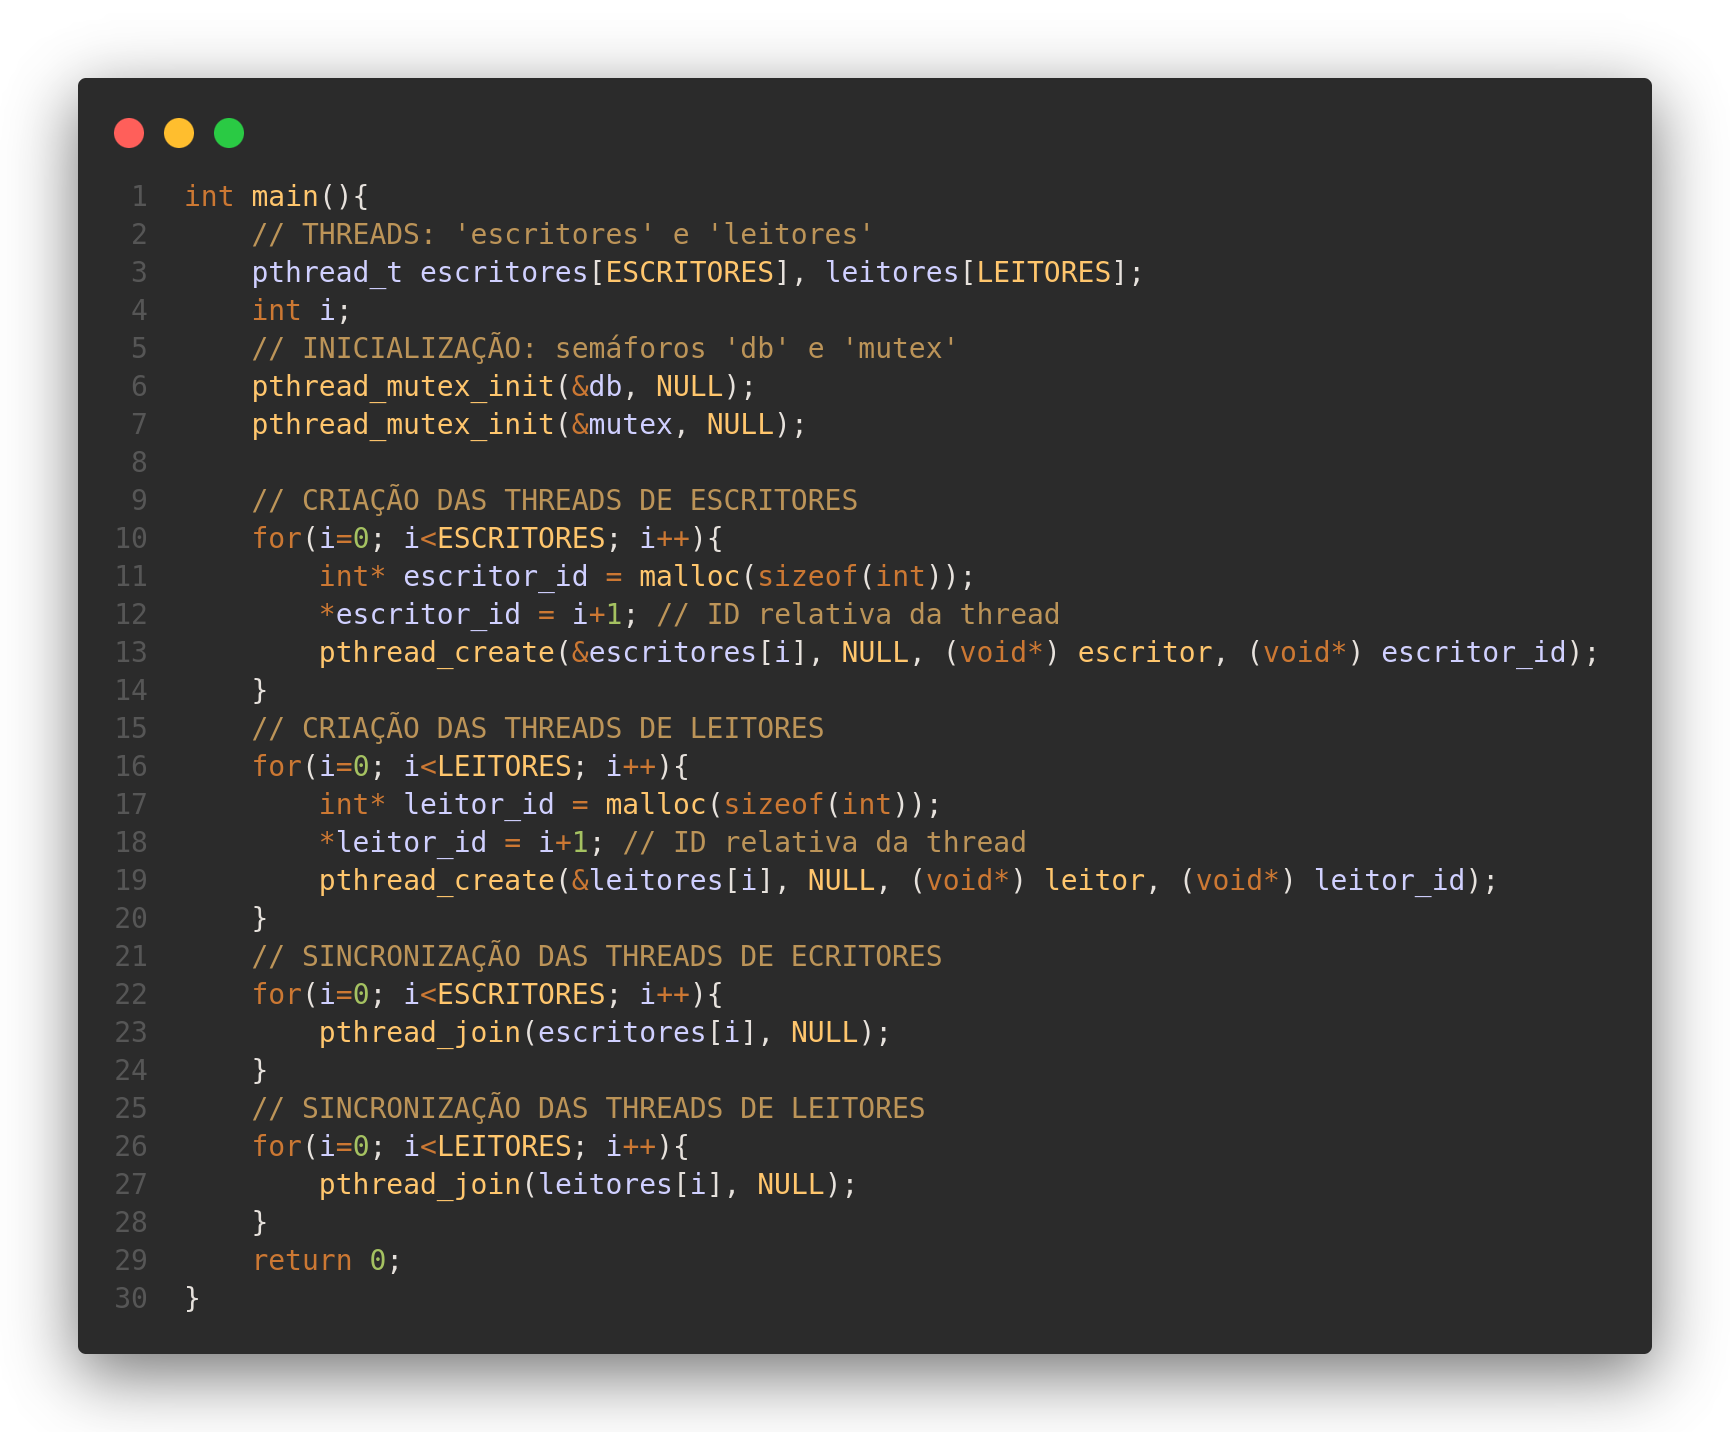
\includegraphics[width=1.0\textwidth]{imagens/leitor_escritor_2.png}
    \caption{Leitor x Escritor: Código em C - Parte II}
    \label{fig:3}
\end{figure}

\begin{figure}[ht]
    \centering
    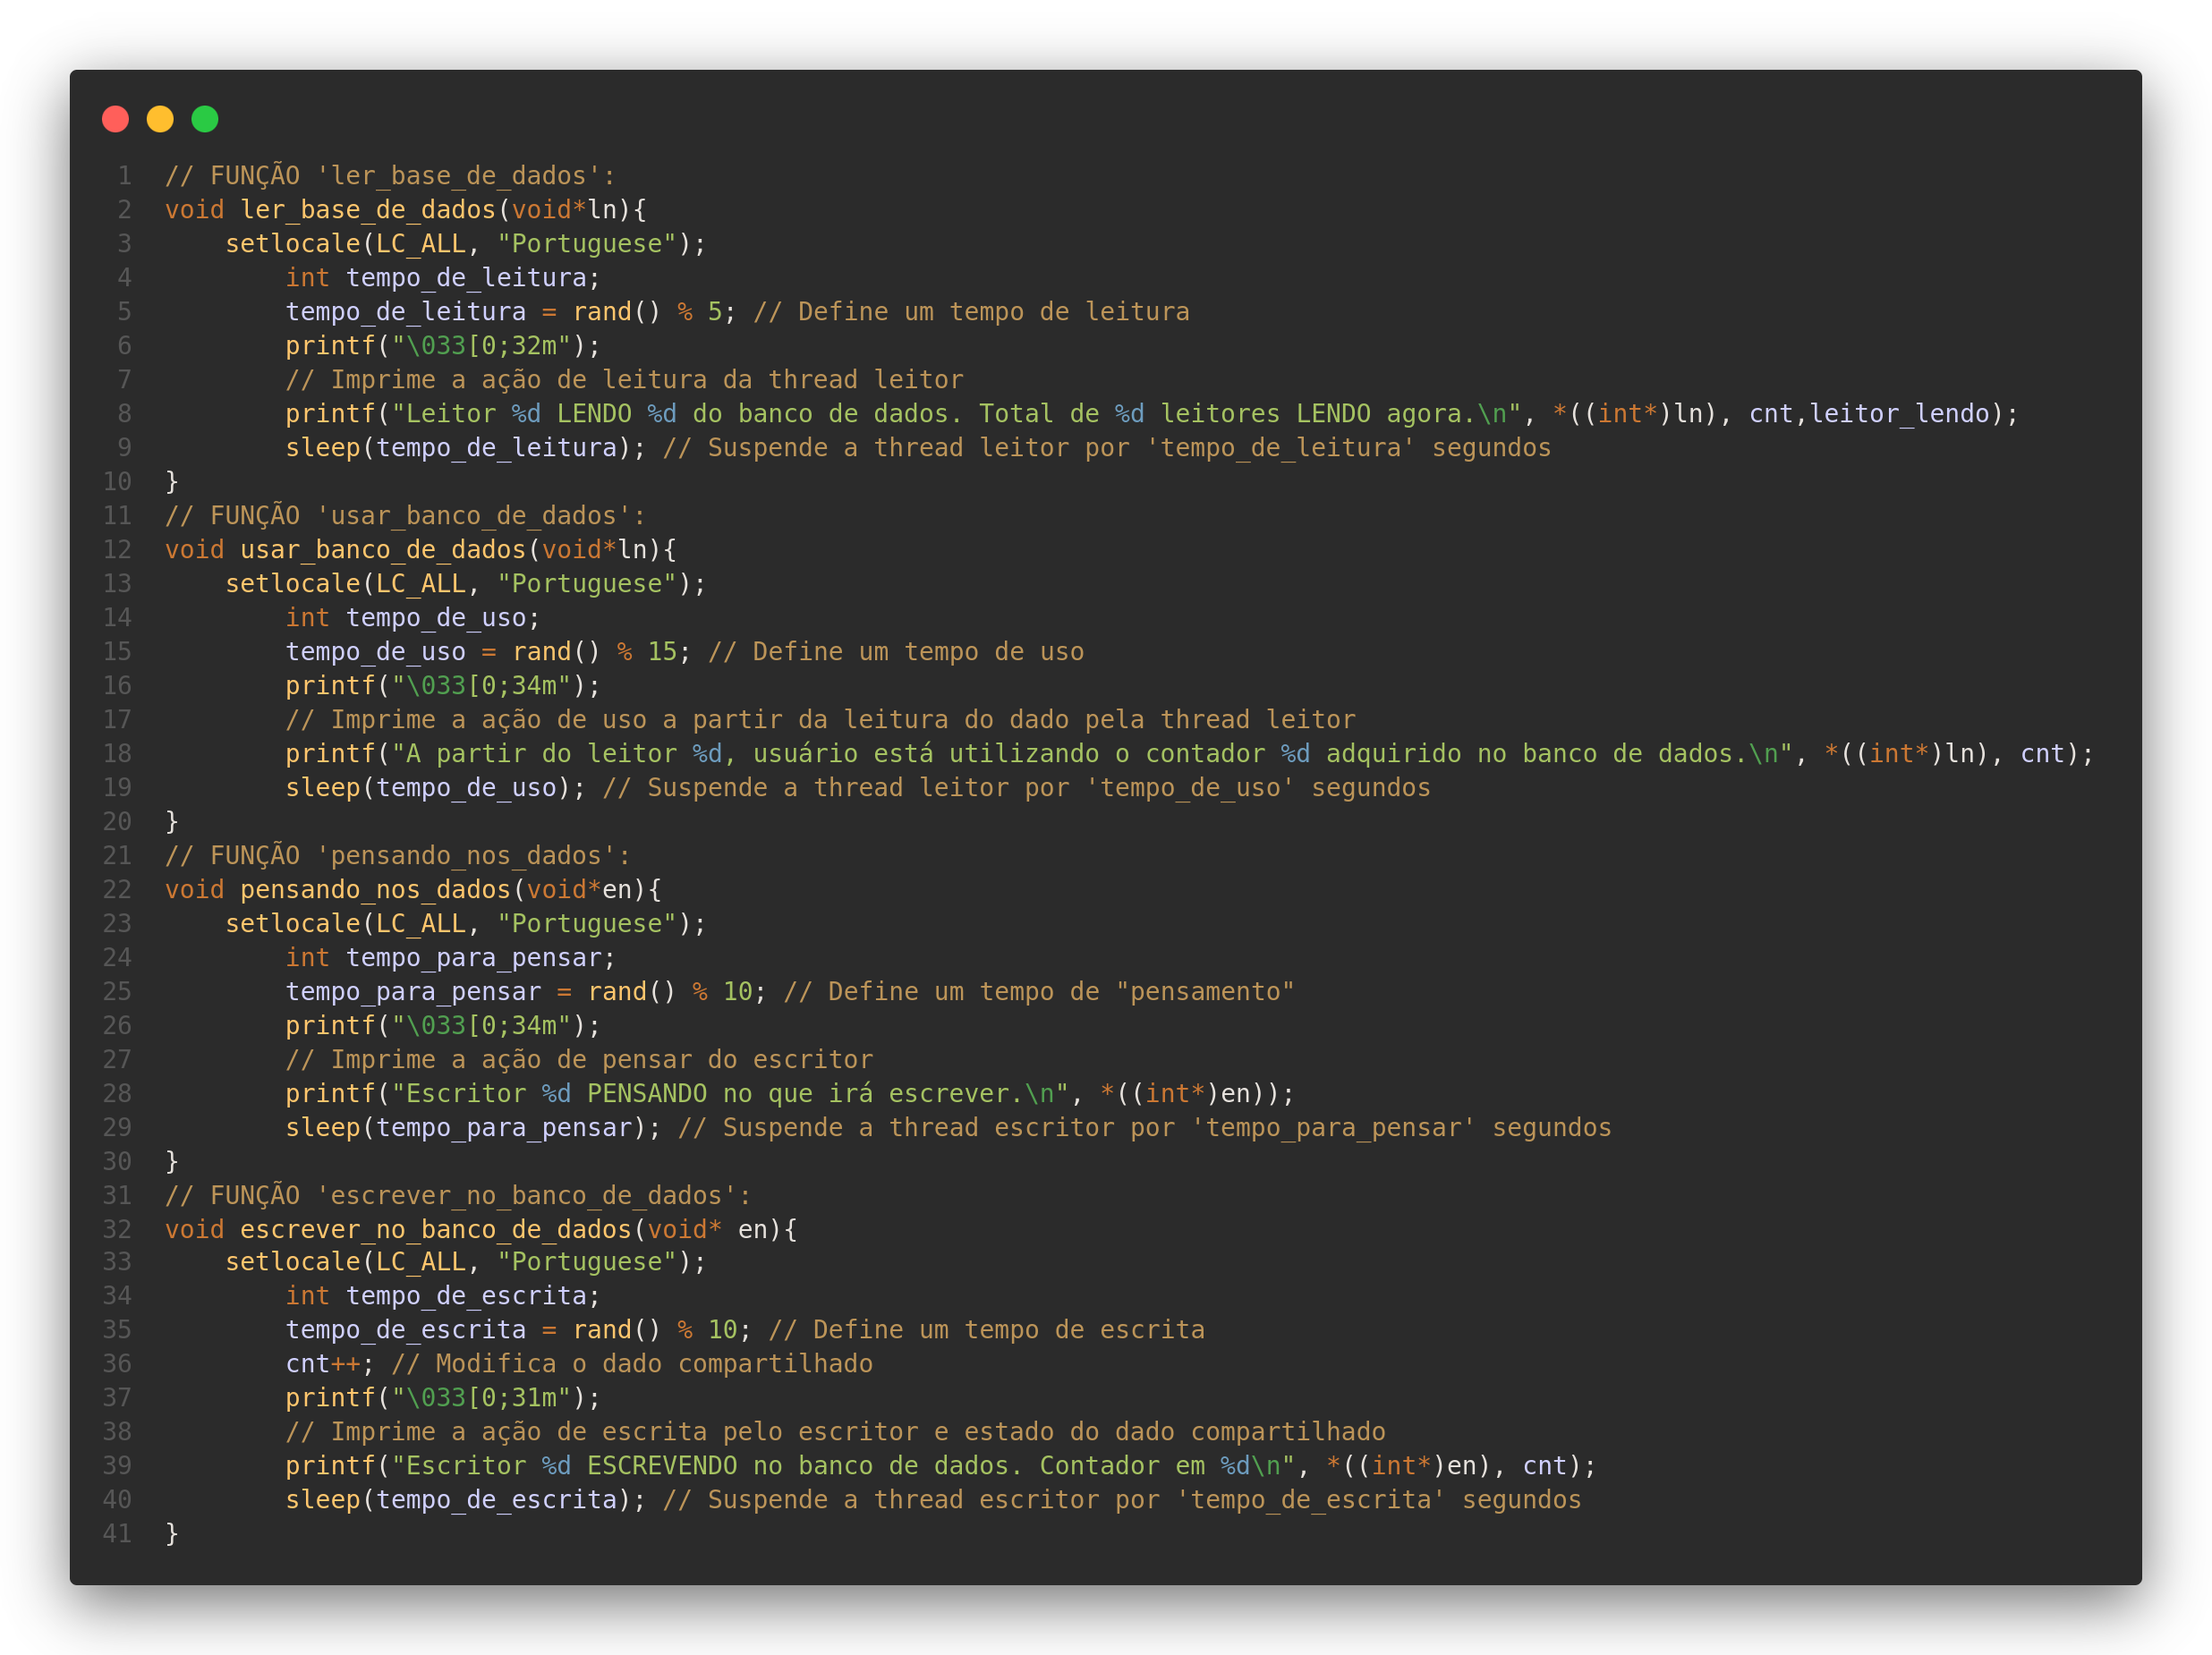
\includegraphics[width=1.0\textwidth]{imagens/leitor_escritor_3.png}
    \caption{Leitor x Escritor: Código em C - Parte III}
    \label{fig:4}
\end{figure}

\clearpage
\section {Conclusão}

O problema Leitor x Escritor é um bom ponto de partida para entendermos como a concorrência entre tarefas é importante e as implicações ao seu respeito. Na situação descrita, foi possível verificar, por meio do código, a relação entre várias tarefas quanto ao compartilhamento e acesso a uma região de memória comum. A coordenação sincronizada do acesso à essa região garante o bom funcionamento do código e da execução dessas tarefas. Para isso, foram utilizados semáforos para o controle do acesso de regiões críticas entre as threads \ovalbox{leitores} e \ovalbox{escritores}, garantindo a exclusão mútua. O entendimento desse tipo de situação é crucial para o controle de acesso em sistemas de dados sincronizados onde leitura e escrita de dados são frequentes.

\chapter{O Jantar dos Filósofos}
\section {Descrição do Problema}

Cinco filósofos estão sentados em uma mesa redonda para jantar. Cada filósofo tem um prato com espaguete à sua frente. Cada prato possui um garfo para pegar o espaguete. O espaguete está muito escorregadio e, para que um filósofo consiga comer, será necessário utilizar dois garfos. Nesse sentido, cada filósofo alterna entre duas tarefas: comer ou pensar. Quando um filósofo fica com fome, ele tenta pegar os garfos à sua esquerda e à sua direita; um de cada vez, independente da ordem. Caso ele consiga pegar dois garfos, ele come durante um determinado tempo e depois recoloca os garfos na mesa. Em seguida ele volta a pensar \cite{jantar-filosofos}. O problema do Jantar dos filósofos modela uma situação de prevenção de deadlock, isto é, quando dois ou mais processos ficam impedidos de continuar seus fluxos execução, ou seja, quando estiverem bloqueados aguardando a liberação de recursos que estão alocados entre eles. Os filósofos e os garfos são analogias para os processos e recursos, respectivamente. Como os recursos são limitados, sem a devida coordenação entre os processos, ou filósofos, pode ocorrer deadlock durante a execução do código. O desafio é propor um algoritmo que implemente cada filósofo de modo que ele execute as tarefas de comer e pensar sem nunca ficar travado. A \textbf{Figura~\ref{fig:jantar_exemplo}} exemplifica a situação onde 5 pratos, para 5 filósofos, estão dispostos à mesa, junto a 5 garfos disponíveis para serem usados.

\begin{figure}
    \centering
    
\includegraphics{imagens/jantar.png}
    \caption{Ilustração do Jantar dos Filósofos}
    \label{fig:jantar_exemplo}
\end{figure}

Portanto, para desenvolver uma solução, é preciso atender às seguintes condições:

\begin{itemize}
    \item Para poder comer, um filósofo deve dispor de 2 garfos;
    \item Cada garfo deve ser controlado de modo que seja utilizado exclusivamente por um filósofo por vez;
    \item Deve-se evitar ao máximo a situação crítica onde cada filósofo detém um garfo, mas não há mais nenhum garfo disponível para nenhum comer, travando a execução dos filósofos;
\end{itemize}

\section{Implementação em C}
\subsection{Contexto}
Cinco threads diferentes, cada uma representando um filósofo, são criadas e concorrem entre si pelo acesso a um recurso limitado (os garfos). Cada thread filósofo alterna entre duas ações: comer e pensar. Para comer, um filósofo precisa acessar dois dos recursos, isto é, dois dos garfos, exclusivamente. Quando não está comendo, o filósofo está automaticamente pensando. A ideia é coordenar as ações dos filósofos, evitando deadlock.
\subsection{Proposta}
A situação que queremos evitar se dá quando cada um dos filósofos aloca um dos recursos pra si ao mesmo tempo. Tendo 5 filósofos e 5 garfos, se essa situação ocorrer, todos eles ficam travados sem retorno à execução, configurando deadlock. 

Para evitar isso de acontecer, a solução proposta, implementada em C, faz uso de semáforos para controlar o acesso à mesa e aos garfos disponíveis. Assim, cada filósofo precisa obrigatoriamente garantir acesso exclusivo a dois garfos para poder comer.
\subsection{Código}

O código-fonte em C utiliza as seguintes bibliotecas:
\begin{itemize}
    \item \textbf{\ovalbox{pthread.h}}: Para criação e gerenciamento de threads e mutexes;
    \item \textbf{\ovalbox{semaphore.h}}: Para implementação de semáforos;
    \item \textbf{\ovalbox{stdio.h}} e \textbf{\ovalbox{stdlib.h}}: Bibliotecas-padrão de entrada e saída;
    \item \textbf{\ovalbox{unistd.h}}: Para o uso de funções como \ovalbox{sleep()};
\end{itemize}

O primeiro trecho de código é descrito a seguir:

\begin{verbatim}
// PROTÓTIPOS: 'filosofos', 'comer' 
void* filosofos(void *);
void* comer(int);

/* DECLARAÇÃO DOS SEMÁFOROS
'filosofo': filósofos na mesa
'garfo': garfos disponíveis na mesa */
sem_t filosofo;
sem_t garfo[5];
\end{verbatim}

Os protótipos das funções \ovalbox{filosofos()} e \ovalbox{comer()} são declarados.

O semáforos \ovalbox{filosofo} e \ovalbox{garfo[]} controlam o acesso à mesa e aos recursos, respectivamente. Observe que \ovalbox{garfo[]} é um conjunto de semáforos, cada um com acesso próprio. 

Tendo essas entidades sido definidas, cada thread filósofo executa a função \ovalbox{filosofos()}, a qual é descrita abaixo:

\begin{verbatim}
// FUNÇÃO 'filosofos':
void* filosofos(void * n){
    int f = *(int *)n; // Conversão do ID da thread filósofo

    while(1){
        sem_wait(&filosofo); // Acessa o semáforo de filósofos
        sem_wait(&garfo[f]); // Acesso ao garfo n
        sem_wait(&garfo[(f+1)%5]); // Acesso ao garfo n + 1

        sleep(2); // Espera de 2 segundos
        comer(f); // Função 'comer' para o filósofo f

        printf("Filósofo %d terminou de comer\n\n", f);
        sem_post(&garfo[(f+1)%5]); // Libera o garfo 'n+1'
        sem_post(&garfo[f]); // Libera o garfo 'n'
        sem_post(&filosofo); // Incrementa o semáforo filosofo
        sleep(5);
    }
}
\end{verbatim}

A função \ovalbox{filosofos()} recebe o argumento \ovalbox{void* n} como identificador da thread filósofo correspondente, e é responsável pela rotina de acesso ao recurso garfo[f], onde \ovalbox{f = *(int*)n}. O fluxo de execução da função se dá conforme o seguinte procedimento:

\begin{enumerate}
    \item Solicita acesso à mesa, pelo semáforo \ovalbox{filosofo}. Tendo acesso, prossegue, senão espera;
    \item Solicita acesso ao primeiro garfo, de posição f, pelo semáforo \ovalbox{garfo[f]};
    \item Tendo acesso, prossegue, senão espera;
    \item Solicita acesso ao segundo garfo, de posição 'f+1', pelo semáforo \ovalbox{garfo[f+1]}. Tendo acesso, prossegue, senão espera;
    \item Executa a ação comer, pela função \ovalbox{comer()};
    \item Libera o garfo de posição 'f', pelo semáforo \ovalbox{garfo[f]};
    \item Libera o garfo de posição 'f+1', pelo semáforo \ovalbox{garfo[f+1]};
    \item Suspende a execução por 5 segundos, pela função \ovalbox{sleep()};
    \item Retorna ao passo 1.
\end{enumerate}
A função \ovalbox{filosofos()} é responsável por chamar a função \ovalbox{comer()}, cujo código é descrito a seguir:

\begin{verbatim}
// FUNÇÃO 'comer': Imprime indicando que o filósofo 'f' está comendo
void* comer(int f){
    sleep(1);
    printf("Filósofo %d está comendo\n",f);
}
\end{verbatim}

A função \ovalbox{comer(int f)} recebe um inteiro \ovalbox{f} como argumento. Nela, a thread é suspensa por 1 segundo, e é impresso na saída uma mensagem indicando que o filósofo 'f' está comendo.

A função principal \ovalbox{main} é responsável por inicializar os semáforos, bem como as threads filósofos (após serem criadas). O código é descrito a seguir:

\begin{verbatim}
int main(){
    int i, a[5];
    pthread_t thread[5];
    // INICIALIZAÇÃO: 'filosofos' sentados à mesa: 5
    sem_init(&filosofo, 0, 4);

    // INICIALIZAÇÃO: cada garfo é disponível a um único filósofo por vez
    for(i = 0; i < 5 ; i++){
        sem_init(&garfo[i], 0, 1); 
    }

    // CRIAÇÃO DAS THREADS
    for(i = 0; i < 5; i++){
        a[i]=i; // Identificação das Threads
        pthread_create(&thread[i], NULL, filosofos, (void *)&a[i]);
    }
    // Sincronização das Threads
    for(i = 0; i < 5; i++){
        pthread_join(thread[i], NULL);
    }
}
\end{verbatim}

O contador \ovalbox{i} é utilizado nos laços 'for' como fator de iteração. O vetor de inteiros \ovalbox{a[]} é utilizado para guardar o id relativo das threads dentro do código.

O semáforo \ovalbox{filosofo} é inicializado em 4, indicando que 5 threads filósofos podem acessá-lo simultaneamente, e é análogo ao acesso à mesa de jantar, como na \textbf{Figura~\ref{fig:jantar_exemplo}}. O conjunto de semáforos \ovalbox{garfo[]} são incializados em 1, indicando exclusividade a um dos filósofos por vez.

As 5 threads filósofos \ovalbox{thread[]} do tipo \ovalbox{pthread\_t} são incializadas, passando o id respectivo ao contador \ovalbox{i}. Logo após, as mesmas são sincronizadas por meio da função \ovalbox{pthread\_join()}. 

Seguindo o fluxo do programa, as threads filósofos executam suas rotinas de acesso aos garfos e execução da ação comer. Na próxima seção será mostrada a saída da execução do código da solução proposta.

O código completo está disponibilizado, juntamente com as instruções, no \href{https://github.com/jvictorferreira3301/Sistemas_Operacionais}{nosso repositório da disciplina}.

\newpage
\subsection{Execução}
A seguir, mostra-se uma captura de saída durante a execução do código \ovalbox{jantar\_filosofos.c}, bem a análise do que pode ser visualizado.

\begin{figure}[h]
    \centering
    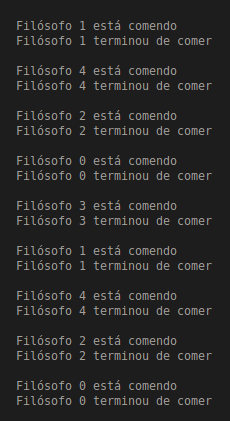
\includegraphics[width=0.5\textwidth]{imagens/out_jantar_filosofos.png}
    \caption{Saída no terminal do código jantar\_filosofos.c}
    \label{fig:out_jantar_filosofos}
\end{figure}

Como mostra a \textbf{Figura~\ref{fig:out_jantar_filosofos}}, Quando um filósofo tem acesso a dois dos semáforos \ovalbox{garfo[]}, executa a função \ovalbox{comer}, que imprime na saída "Filósofo (id) está comendo". Terminando a execução da função, é impresso "Filósofo (id) terminou de comer", indicando que o filósofo terminou de comer. Pela saída, é possível observar a existência de rotatividade e controle no acesso ao recurso limitado (garfos), enfatizando que todas as threads filósofos, enumeradas de 0 a 4, são executadas, com sucesso, pelo menos uma vez. Isso demonstra que a solução implementada obteve sucesso em atender aos requisitos descritos pelo problema.

\subsection{Análise}
\subsubsection{Da solução implementada}
O uso do conjunto de semáforos \ovalbox{garfo[]} como uma lista de semáforos é um uso interessante dessa estrutura, aglomerando os garfos como recurso, mas também diferenciando cada garfo individualmente, com acesso próprio. 

Para executar a ação \ovalbox{comer}, cada filósofo deve acessar dois garfos, \ovalbox{garfo[i]} e \ovalbox{garfo[i+1]}, simultaneamente, garantindo, desde o início, certa ordem de chegada ao recurso. Como o acesso se dá aos garfos próximos de um filósofo  \ovalbox{f}, dois filósofos próximos exercem exclusão mútua, contribuindo para a prevenção de deadlock.

\subsubsection{De possíveis melhorias}

A solução proposta é suficiente ao atingir o objetivo principal de prevenção de deadlock. Por outro lado, salienta-se algumas possíveis melhorias a serem implementadas no código:
\begin{enumerate}
    \item O código não implementa, de fato, uma função \ovalbox{pensar}. Logo, seria interessante adicionar um procedimento do tipo. 
\end{enumerate}

\clearpage
\section{Capturas da IDE mostrando o código}
Nesta seção serão apresentadas capturas da tela da IDE mostrando os códigos apresentados acima, que se encontram, também disponíveis no
\href{https://github.com/jvictorferreira3301/Sistemas_Operacionais}{nosso repositório da disciplina}.
\begin{figure}[h]
    \centering
    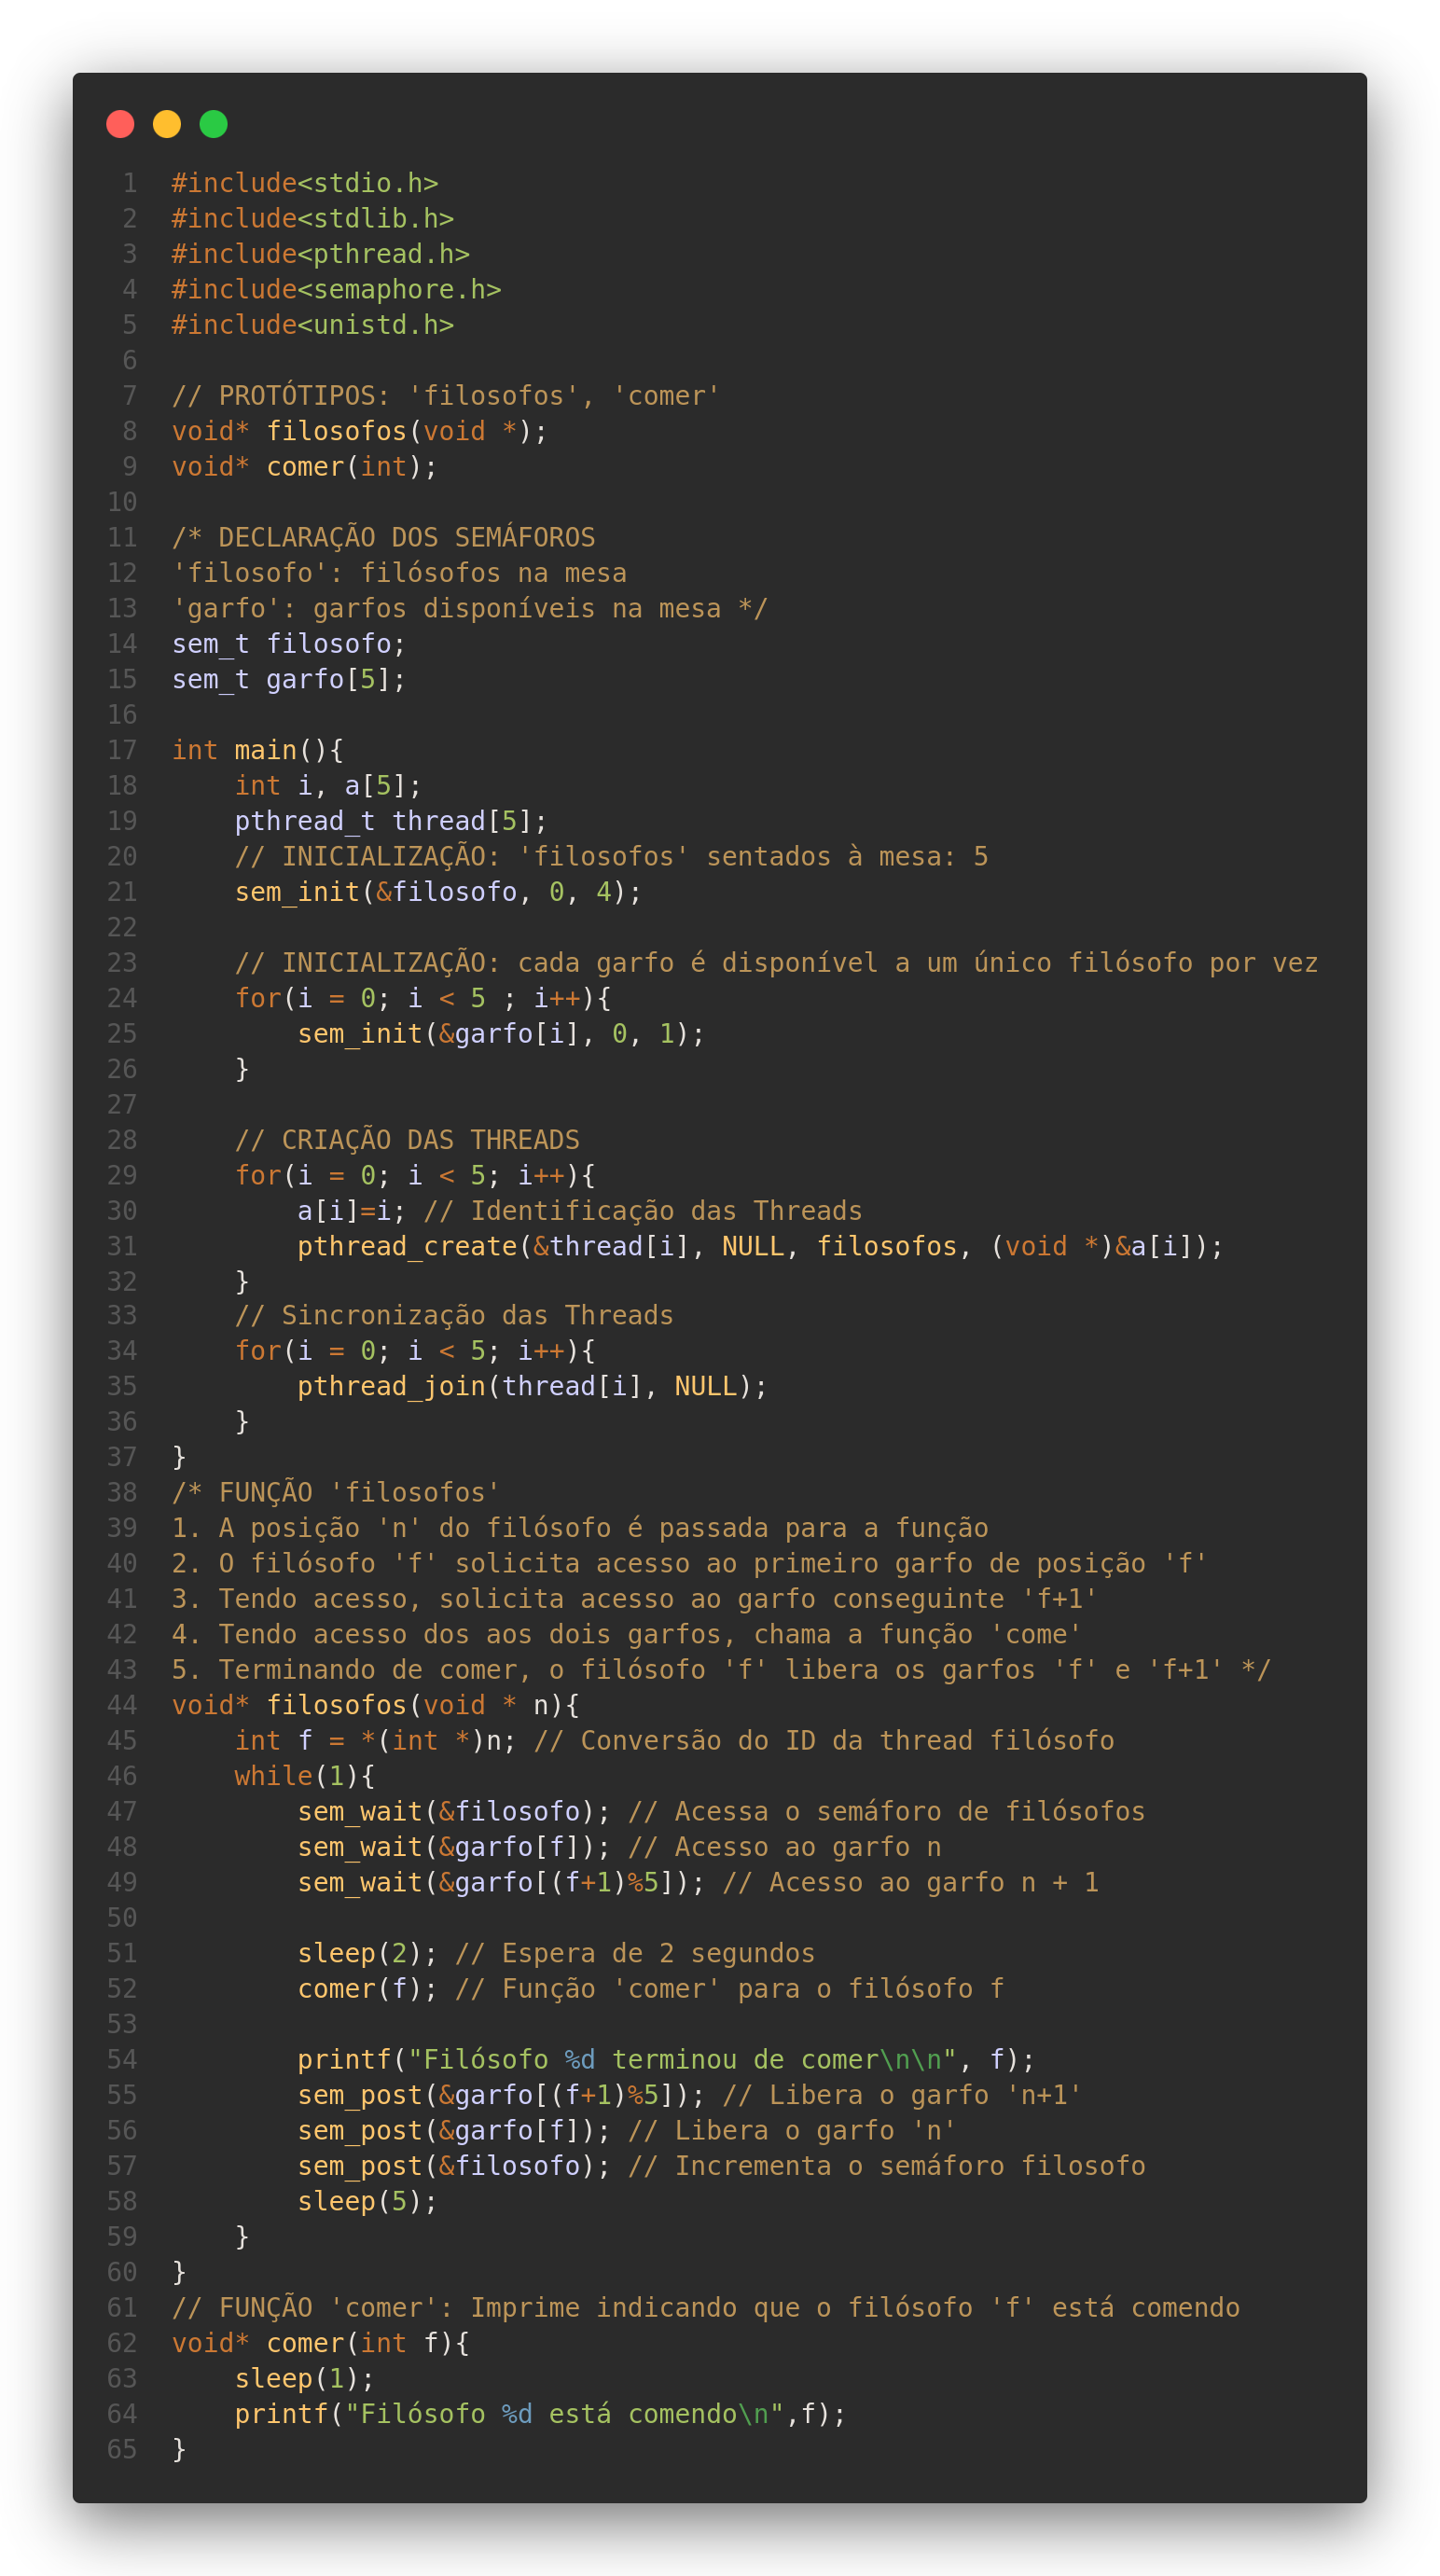
\includegraphics[width=0.7\textwidth]{imagens/jantar_filosofos.png}
    \caption{O Jantar dos Filósofos: Código em C}
    \label{fig:jantar_filosofos}
\end{figure}
\clearpage
\section{Conclusão}

A problema do Jantar dos Filósofos é um interessante paradigma de coordenação de acesso ordenado ao recurso para prevenção de deadlock. Tendo em vista que este é um problema frequente, difícil de lidar e de prever, o entendimento de seu contexto é importante durante o desenvolvimento de pensamento lógico para solução de problemas em sistemas operacionais.

A solução apresentada neste trabalho propõe um uso interessante de uma lista semáforos como mediadores de acesso, sendo os próprios semáforos analogias para o recurso limitado "garfos". É interessante observer que, não só o uso da lista, mas também a necessidade de acesso simultâneo a dois elementos conseguintes da mesma, uma ideia interessante que pode ser utilizada e mais situações.

Contudo, a solução proposta lidou bem com a situação problema e contribui para o entendimento dos temas discutidos neste capítulo.

\chapter{Problema do Produtor x Consumidor}
\section{Descrição do Problema}
O problema do produtor e consumidor, também referido como Bounded Buffer Problem (BBP), consiste em um desafio de sincronização de duas ou mais threads (tarefas) concorrentes que têm acesso a um mesmo recurso do programa que está sendo executado. O fato de o recurso estar sendo compartilhado, implica na possibilidade de conflitos entre as threads que disputam pelo controle da CPU para acessar esse mesmo recurso.

No caso do BBP, o recurso disputado é um buffer de memória (um vetor), de tamanho limitado/fixo, daí o motivo do nome. O produtor é o responsável por enfileirar novos jobs ou dados nesse buffer, e o consumidor assume a responsabilidade de extrair esses dados do buffer. Porém o seguinte problema poderá emergir: E se o produtor produzir muito rápido, e o consumidor não for capaz de acompanhá-lo? Se isso acontecer, o produtor irá descartar todos os novos itens produzidos, até que haja espaço novamente no buffer, ou seja, dados serão perdidos. Mas ainda podemos contornar esse problema, o que discutiremos na seção a seguir \cite{produtor-consumidor}.

A \textbf{Figura~\ref{fig:ex_prod_cons}} abaixo exemplifica a situação problema, onde um buffer finito é utilizado como canal entre as entidades produtor e consumidor.

\begin{figure}[h]
    \centering
    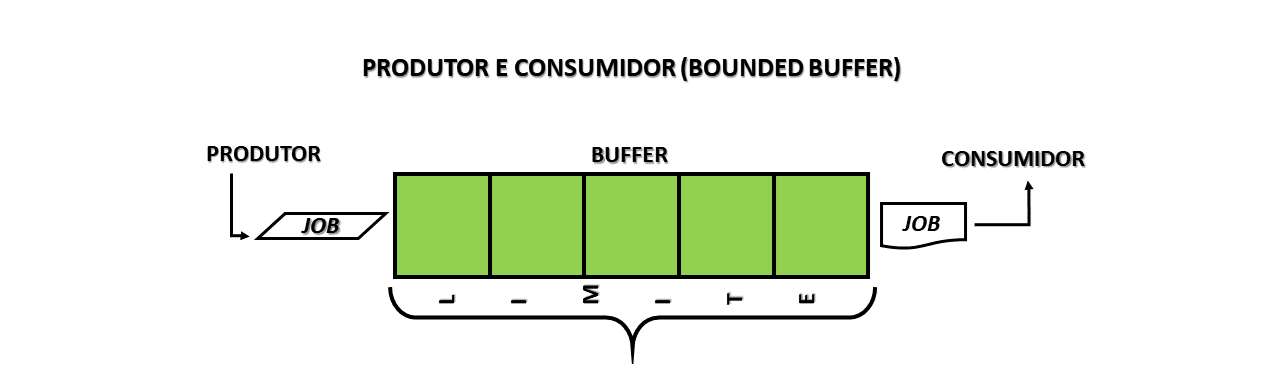
\includegraphics[width=1.0\textwidth]{imagens/ex_prod_cons.png}
    \caption{Produtor x Consumidor: Exemplo ilustrativo}
    \label{fig:ex_prod_cons}
\end{figure}

Portanto, para desenvolver um solução para esse problema, devemos atender às seguintes condições:
\begin{itemize}
    \item Os produtores devem adicionar itens ao buffer enquanto houver espaço. Caso não haja, devem esperar até que itens sejam consumidos, e espaço seja liberado;
    \item Os consumidores devem consumir itens do buffer enquanto tiverem itens a serem consumidos. Caso não haja, devem esperar serem produzidos e adicionados ao buffer;
    \item Deve-se garantir exclusão mútua de acesso ao buffer, para evitar condição de corrida.
\end{itemize}

\section{Implementação em C}
\subsection{Contexto}
Um buffer de tamanho pré-definido é compartilhado entre algumas threads. 5 consumidores e 5 produtores. Produtores produzem itens que serão alocados em uma das posições do buffer, e consumidores retiram informação de determinada posição do mesmo e a consomem. É necessário coordenar o acesso ao buffer para evitar perda de dados e sobrecarregamento do buffer, bem como a ociosidade das threads e condição de corrida.
\subsection{Proposta}
A solução implementada em C faz uso de semáforos para controlar o estado do buffer, garantindo que haja espaço para ser preenchido com novos dados, quando necessário, bem como que haja dados a serem lidos do buffer. Além disso, é utilizado um mutex para garantir a exclusão mútua ao buffer, onde apenas uma threads tem acesso ao buffer por vez, seja para produzir ou consumir.
\subsection{Código}
O código-fonte em C utiliza as seguintes bibliotecas:
\begin{itemize}
    \item \textbf{\ovalbox{pthread.h}}: Para criação e gerenciamento de threads e mutexes;
    \item \textbf{\ovalbox{semaphore.h}}: Para implementação de semáforos;
    \item \textbf{\ovalbox{stdio.h}} e \textbf{\ovalbox{stdlib.h}}: Bibliotecas-padrão de entrada e saída;
\end{itemize}

A priori, temos o seguinte trecho de código:
\begin{verbatim}
#include <pthread.h>
#include <semaphore.h>
#include <stdlib.h>
#include <stdio.h>

// DEFINIÇÃO DE MACROS
#define Maximo 5 // Número máximo de iterações
#define TBuffer 5 // Tamanho do Buffer

// PROTÓTIPOS: 'produtor()' e 'consumidor()' 
void *produtor(void *pno);
void *consumidor(void *cno);
// SEMÁFOROS:
sem_t vazio; // 'vazio': semáforo para indicar se 
                pode adicionar um novo item ao buffer
sem_t cheio; // 'cheio': semáforo para indicar 
                se pode consumir um item do buffer 
// VARIÁVEIS DE CONTROLE:
int entrando = 0; // 'entrando': Variável auxiliar para indexação
int saindo = 0; // 'saindo':  Variável auxiliar para indexação
int buffer[TBuffer]; 
pthread_mutex_t mutex; // Mutex para exclusão mútua ao buffer 
\end{verbatim}

Primeiramente, define-se os macros para o controle máximo de iterações, \ovalbox{Maximo}, dos produtores e consumidores, bem com de controle do tamanho do buffer \ovalbox{TBuffer}. Os protótipos das funções características de produtor e consumidor, \ovalbox{produtor()} e \ovalbox{consumidor()}, respectivamente, são definidos logo após. 

Os semáforos \ovalbox{vazio} e \ovalbox{cheio} são responsáveis por controlar o acesso ao buffer quanto à possibilidade de adicionar um item ao buffer ou consumir um item dele, respectivamente.

As variáveis de controle \ovalbox{entrando} e \ovalbox{saindo} são utilizadas como auxílio para a indexação da posição do item que será adicionado ou retirado do buffer.

Por fim, um mutex \ovalbox{mutex} garante acesso exclusivo ao buffer por uma das threads. Para acessar os recursos descritos acima, as funções \ovalbox{produtor} e \ovalbox{consumidor} são definidas, e serão descritas abaixo:

\begin{verbatim}
// FUNÇÃO 'produtor()':
void *produtor(void *pno){
    int item;
    for(int i = 0; i < Maximo; i++) {
        item = rand() % 10; // Produz um item aleatório
        sem_wait(&vazio); // Solicita acesso ao semáforo 'vazio'
        pthread_mutex_lock(&mutex); // Solicita lock ao mutex 
        buffer[entrando] = item; // Adiciona 'item' ao buffer em 'entrando'
        printf("Produtor %d: Insere item %d em %d\n", 
                *((int*)pno),buffer[entrando],entrando);
        entrando = (entrando+1)%TBuffer; // 'entrando' é incrementado 
        pthread_mutex_unlock(&mutex); // // O mutex é liberado
        sem_post(&cheio); // O semáforo 'cheio' é incrementado
    }
}
\end{verbatim}

A função \ovalbox{produtor} recebe \ovalbox{void*pno} como identificador da thread produtor e utiliza-o para impressão na saída. A variável  \ovalbox{item} representa o dado que será produzido e posto no buffer. A função executa conforme o seguinte procedimento:

\begin{enumerate}
    \item Inicializa a variável \ovalbox{item} e \ovalbox{i = 0};
    \item Se \ovalbox{i <= Maximo}, prossegue, senão encerra;
    \item Produz um item aleatório, atribuindo um inteiro entre 0 e 10 à variável \ovalbox{item};
    \item Solicita acesso ao semáforo \ovalbox{vazio}. Se tiver espaço disponível no buffer, prossegue, senão espera;
    \item Solicita acesso exclusivo ao buffer, pelo mutex \ovalbox{mutex};
    \item Adiciona \ovalbox{item} na posição \ovalbox{entrando} do buffer;
    \item Incrementa \ovalbox{entrando};
    \item Libera o mutex \ovalbox{mutex};
    \item Incrementa o semáforo \ovalbox{cheio};
    \item Incrementa \ovalbox{i};
    \item Retorna ao passo 2.
\end{enumerate}

A seguir, temos a função \ovalbox{consumidor()}:

\begin{verbatim}
    // FUNÇÃO CONSUMIDOR
void *consumidor(void *cno){
    for(int i = 0; i < Maximo; i++) {
        sem_wait(&cheio); // Solicita acesso ao semáforo 'cheio'
        pthread_mutex_lock(&mutex); // Solicita lock ao mutex 
        int item = buffer[saindo]; // "consome" o item da posição 'saindo' 
        printf("Consumidor %d: Remove item %d de %d\n",
                            *((int *)cno),item, saindo);
        saindo = (saindo+1)%TBuffer; // 'saindo' é incrementado 
        pthread_mutex_unlock(&mutex); // Libera o mutex
        sem_post(&vazio); // O semáforo 'vazio' é incrementado
    }
}
\end{verbatim}

A função recebe \ovalbox{void*cno} como parâmetro para representar o id relativo ao código da thread consumidor, e seu procedimento é descrito a seguir:
\begin{enumerate}
    \item Inicializa a variável \ovalbox{i};
    \item Se \ovalbox{i <= Maximo}, prossegue, senão encerra;
    \item Solicita acesso ao semáforo \ovalbox{cheio}. Se tiver pelo menos um item a ser consumido, prossegue, senão espera;
    \item Solicita acesso exclusivo ao buffer, pelo mutetx \ovalbox{mutex}. Tendo acesso, prossegue, senão espera;
    \item Lê um item de posição \ovalbox{saindo} do buffer;
    \item Incrementa \ovalbox{saindo};
    \item Libera o mutex \ovalbox{mutex};
    \item Incrementa o semáforo \ovalbox{vazio};
    \item Incrementa \ovalbox{i};
\end{enumerate}

A função principal \ovalbox{main()} é responsável por inciar os semáforos, bem como criar, inicializar e sincronizar as threads \ovalbox{pro} e \ovalbox{con}, representando os produtores e consumidores, respectivamente. O trecho de código  da função \ovalbox{main()} é descrito a seguir:

\begin{verbatim}
int main(){
    /* VARIÁVEIS 
    Threads: 'pro' produtores, 'con' consumidores */
    pthread_t pro[5],con[5];
    // Inicialização dos semáforos
    pthread_mutex_init(&mutex, NULL);
    sem_init(&vazio,0,TBuffer);
    sem_init(&cheio,0,0);
    // Identificação das Threads
    int a[5] = {1,2,3,4,5};

    // Loop de criação das Threads
    for(int i = 0; i < 5; i++) {
        pthread_create(&pro[i], NULL, (void *)produtor, (void *)&a[i]);
    }
    for(int i = 0; i < 5; i++) {
        pthread_create(&con[i], NULL, (void *)consumidor, (void *)&a[i]);
    }
    // Junção das Threads
    for(int i = 0; i < 5; i++) {
        pthread_join(pro[i], NULL);
    }
    for(int i = 0; i < 5; i++) {
        pthread_join(con[i], NULL);
    }
    // Encerramento dos semáforos
    pthread_mutex_destroy(&mutex);
    sem_destroy(&vazio);
    sem_destroy(&cheio);
    return 0;
}
\end{verbatim}

As threads de produtores, \ovalbox{pro[5]}, e consumidores, \ovalbox{con[5]}, do tipo \ovalbox{pthread\_t} são criadas. Os semáforos \ovalbox{vazio} e \ovalbox{cheio} são inicializados em \ovalbox{TBuffer} e 0, respectivamente, indicando que, no início, o buffer está vazio. Para identificar as threads, é utilizado um vetor de inteiros \ovalbox{a[5]}, que é passado como argumento à função \ovalbox{pthread\_create()}, responsável por criar as threads \ovalbox{pro} e \ovalbox{con}, que executarão as rotinas de produtor e consumidor. Logo após, a função \ovalbox{pthread\_join()} é utilizar para auxiliar na sincronização na execução das threads. Tendo encerrado a execução geral, destrói os semáforos e o mutex, por meio das funções \ovalbox{pthread\_mutex\_destroy()} e \ovalbox{sem\_destroy()}.

O código completo está disponibilizado, juntamente com as instruções, no \href{https://github.com/jvictorferreira3301/Sistemas_Operacionais}{nosso repositório da disciplina}.


\subsection{Execução}
A seguir, mostra-se algumas capturas de saída durante a execução do código \ovalbox{jantar\_filosofos.c}, bem a análise do que pode ser visualizado.
\begin{figure}[h]
    \centering
    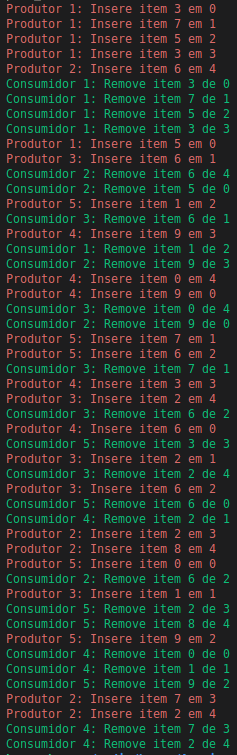
\includegraphics[width=0.4\textwidth]{imagens/out_prod_cons.png}
    \caption{Saída no terminal do código prod\_cons.c}
    \label{fig:out_prod_cons}
\end{figure}

Como mostra a \textbf{Figura~\ref{fig:out_prod_cons}}, os produtores modificam o valor nas cinco posições do vetor \ovalbox{buffer}; esse processo é análogo à ação de produzir e adicionar itens, que confere aos produtores. Assim que adquirem acesso ao buffer, os consumidores leem as posições do buffer, procedimento análogo a "retirar e consumir". Essas ações são impressas na saída indicando a iteração respectiva de cada thread, até que se chegue no máximo de iterações.

\subsection{Análise}
\subsubsection{Da solução implementada}
A solução proposta faz uso de dois semáforos diferentes, \ovalbox{vazio} e \ovalbox{cheio}, para indicar o estado do buffer, e são incrementados e decrementados inversamente ao outro. Isso contribui para a coordenação e acesso ao buffer entre produtores e consumidores, dividindo o controle de acesso, porém ambas com o mesmo intuito. Essa é uma proposta interessante e que pode ser aproveitada em outras situações.

Pela execução do código \ovalbox{prod\_cons.c}, é possível ver que a solução tem êxito em satisfazer os requisitos propostos, coordenação de maneira efetiva as ações entre produtores e consumidores.

\subsubsection{De possíveis melhorias}
A solução proposta no código \ovalbox{prod\_cons.c} soluciona o problema apresentado. Por outro lado, salienta-se possíveis melhorias a serem implementadas:
\begin{enumerate}
    \item  O código tem um número de iterações limitado. É possível torná-lo infinito, tomando devido cuidado com a indexação de acesso ao buffer.
\end{enumerate}

\section{Capturas da IDE mostrando o código}
Nesta seção serão apresentadas capturas da tela da IDE mostrando os códigos apresentados acima, que se encontram, também disponíveis no
\href{https://github.com/jvictorferreira3301/Sistemas_Operacionais}{nosso repositório da disciplina}.

\begin{figure}[h]
    \centering
    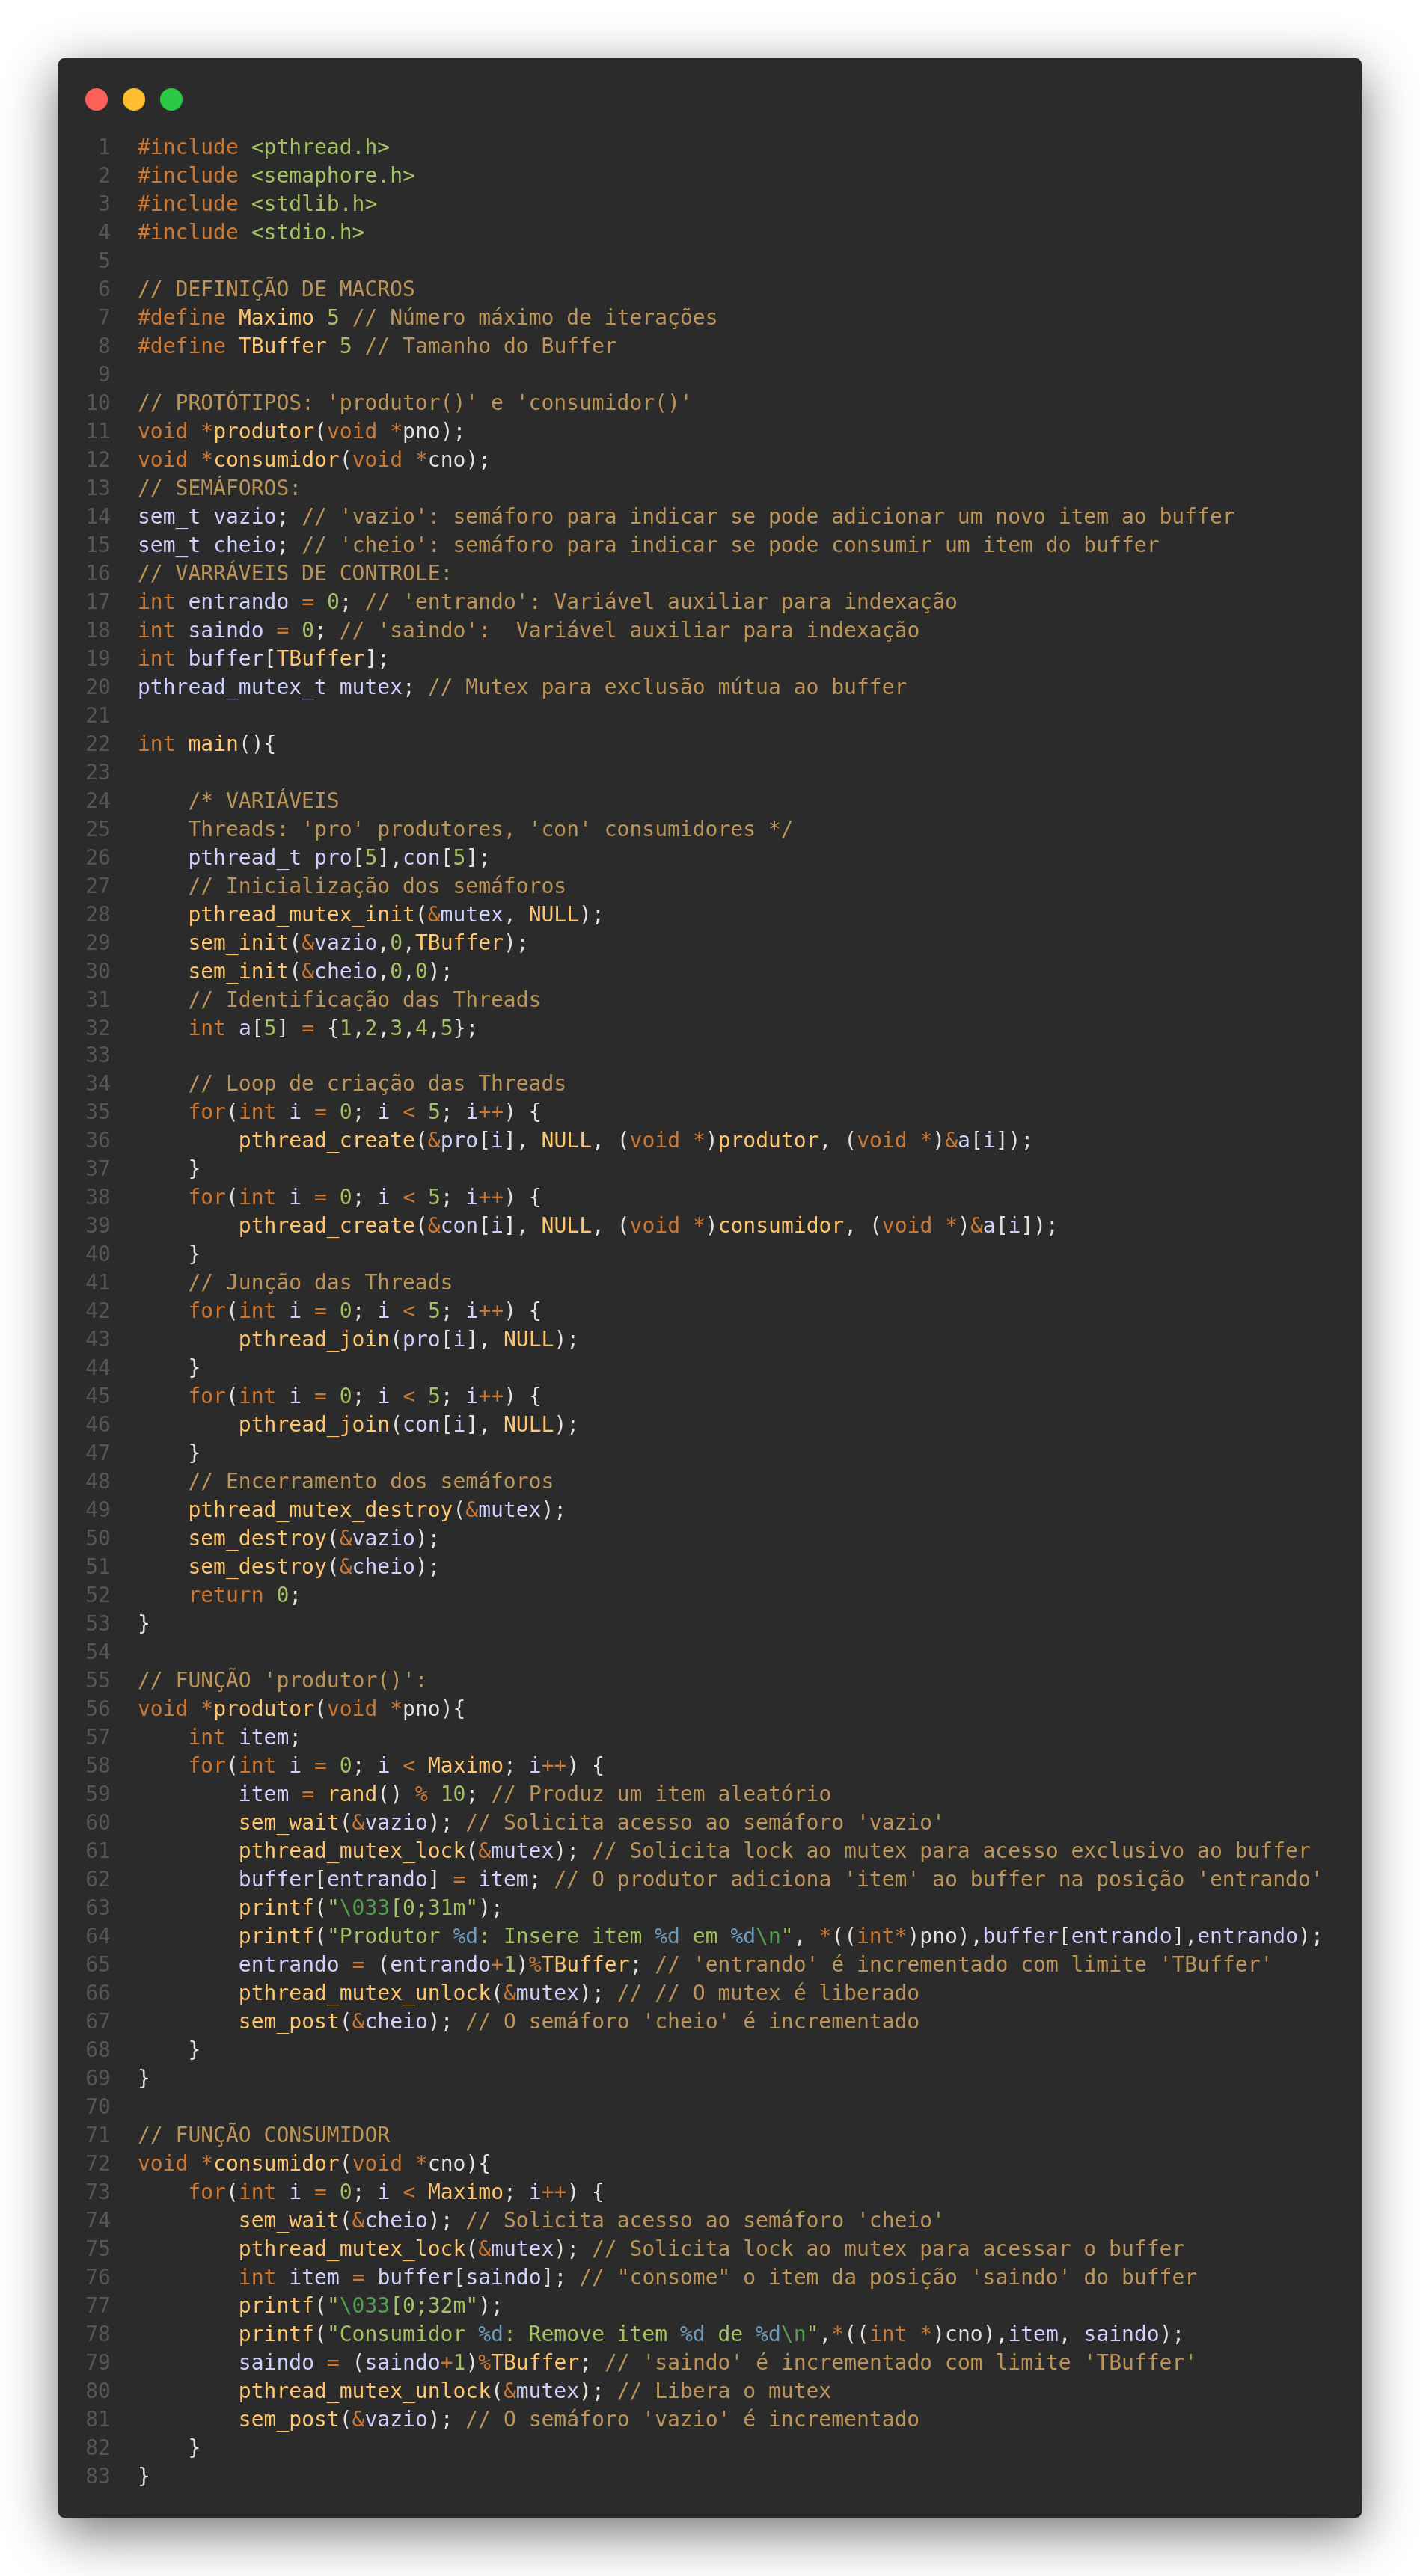
\includegraphics[width=0.8\textwidth]{imagens/prod_cons.png}
    \caption{Produtor x Consumidor: Código em C}
    \label{fig:prod_cons}
\end{figure}

\clearpage
\section{Conclusão}

O Problema do Produtor x Consumidor modela uma situação recorrente de compartilhamento de um canal de buffer importante para o estudo em sistemas operacionais. São frequentes as situações em que processos dependem da saída de outros processos, sendo crucial a coordenação entre eles para o fluxo de execução.

A solução proposta controla não só o acesso ao buffer, mas também o estado do buffer, por meio de semáforos, ajustando as iterações e garantindo acessos exclusivos durante o fluxo de execução.

Concluindo, a solução proposta lida bem o problema discutido e auxilia no entendimento de coordenação de acesso a um canal compartilhado (buffer), discutido acima.


\chapter{O Problema do Barbeiro Dorminhoco}
\section{Descrição do Problema}
O problema do barbeiro dorminhoco é um problema clássico de comunicação inter-processo e sincronização entre múltiplos processos. O problema é análogo a manter o barbeiro ocupado enquanto há clientes, e descansando quando não há nenhum (fazendo isso de uma maneira ordenada). O barbeiro e seus clientes correspondem aos processos mencionados acima \cite{barbeiro-dorminhoco}. 

Eis a situação: Em uma barbearia há um barbeiro, que está destinado a duas ações - cortar o cabelo de um cliente ou descansar (dormir). Caso não haja clientes na barbearia, o barbeiro se mantém dormindo, se não, corta o cabelo de um dos clientes nas n cadeiras disponíveis no estabelecimento. Os clientes, conforme vão chegando, devem verificar se há cadeiras disponíveis para sentar, se conseguirem sentar, esperam até que o barbeiro termine de cortar o cabelo do cliente anterior. Se não houver nenhuma cadeira disponível, isto é, o salão está cheio, o cliente deve ir embora. 

O problema é programar o barbeiro e os clientes sem cair em condições de disputa. Esse problema é semelhante a situações com várias filas, como uma mesa de atendimento de telemarketing com diversos atendentes e com um sistema computadorizado de chamadas em espera, atendendo a um número limitado de chamadas que chegam \cite{barbeiro-dorminhoco}.

Para desenvolver uma solução para esse problema, devemo-nos atentar para as seguintes condições:
\begin{itemize}
    \item O barbeiro deve permanecer ocupado enquanto houver clientes esperando;
    \item Um cliente que chegar deve ter acesso ao barbeiro para ter o cabelo cortado, entrando em estado de espera caso o barbeiro esteja ocupado;
    \item Se a barbearia estiver cheia, o cliente que chegar deve ir embora.
\end{itemize}

\section{Implementação em C}
\subsection{Contexto}
Na barbearia, há uma thread barbeiro que altera entre dormir e corta cabelo. Tendo clientes na barbearia, devemos manter o barbeiro ocupado o tempo todo. As threads clientes, por outro lado, chegam na barbearia e devem esperar em uma das cadeiras, se disponíveis, até serem atendidos. Se não conseguirem sentar em nenhuma cadeira, devem ir embora, pois a barbearia está cheia. A tarefa é utilizar recursos para coordenar a atividade do barbeiro e dos clientes para que não haja condição de corrida.

\subsection{Proposta}
A proposta é fazer uso de semáforos para controlar a disponibilidade da barbeiro e das cadeiras, bem como uma variável contador de clientes esperando. Assim, podemos garantir o controle de acesso aos recursos compartilhados essas tarefas barbeiro e cliente.

\subsection{Código}
O código-fonte em C utiliza as seguintes bibliotecas:
\begin{itemize}
    \item \textbf{\ovalbox{pthread.h}}: Para criação e gerenciamento de threads e mutexes;
    \item \textbf{\ovalbox{semaphore.h}}: Para implementação de semáforos;
    \item \textbf{\ovalbox{stdio.h}} e \textbf{\ovalbox{stdlib.h}}: Bibliotecas-padrão de entrada e saída;
    \item \textbf{\ovalbox{unistd.h}}: Para o uso de funções como \ovalbox{sleep()};
    \item \textbf{\ovalbox{locale.h}}: Para impressão de saída em língua portuguesa.
\end{itemize}

A primeiro trecho de código é descrito a seguir:
\begin{verbatim}
#include <stdio.h>
#include <unistd.h>
#include <stdlib.h>
#include <pthread.h>
#include <semaphore.h>
#include <locale.h>

// DEFINIÇÃO DE MACROS
#define CHAIRS 5 // Número de cadeiras para os clientes à espera
#define TRUE 1 // Estado padrão

sem_t clientes; // 'clientes': Número de cliente à espera de atendimento 
sem_t barbeiros; // 'barbeiros': Número de barbeiros à espera de clientes 
sem_t mutex; // 'mutex': Garante acesso exclusivo à 'esperando'
sem_t cliente_cortando_mutex; // Garante exclusão mútua à 'cliente_cortando'
int esperando = 0; // Clientes que estão esperando (não estão cortando) 
int count = 0; // Variável auxiliar para contagem no loop 'while(count < 100)'
int cliente_cortando = 0; // Variável auxiliar de indexação

// PROTÓTIPOS
void* barbeiro(); // Função padrão dos barbeiros
void* cliente(void* id); // Função padrão dos clientes
void cortar_cabelo(); // Indica que o barbeiro está cortando o cabelo
void chegada_cliente(); // Indica a chegada de um novo cliente
void conseguir_corte(); // Indica o que um cliente conseguiu acesso ao barbeiro
void desistir_corte(); // Indica que um cliente desistiu de cortar o cabelo
\end{verbatim}

Os macros \ovalbox{CHAIRS} e \ovalbox{TRUE} definem o número de cadeiras da barbearia e um estado-padrão 1.

Os semáforos \ovalbox{clientes} e \ovalbox{barbeiros} controlam o número de clientes que chegam na barbearia e o estado do barbeiro, dormindo ou cortando cabelo.

O mutex \ovalbox{mutex} garante acesso exclusivo à variável \ovalbox{esperando}, que representa o número de cliente esperando atendimento e, se maior que \ovalbox{CHAIRS}, indica que a barbearia está cheia. A variável \ovalbox{cliente\_cortando} identifica o cliente que está sendo atendido pelo barbeiro, e é utilizada para impressão na saída.

Os protótipos das funções utilizadas no código são descrita como segue:

\begin{enumerate}
    \item \ovalbox{barbeiro()}: Função padrão dos barbeiros;
    \item \ovalbox{cliente(void*id)}: Função padrão dos clientes.
    \item \ovalbox{cortar\_cabelo()}: Indica que o barbeiro está cortando cabelo;
    \item \ovalbox{chegada\_cliente()}: Indica a chegada de um novo cliente;
    \item \ovalbox{conseguir\_corte()}: Indica o que um cliente conseguiu acesso ao barbeiro;
    \item \ovalbox{desistir\_corte()}: Indica que o cliente desistiu de cortar o cabelo.
\end{enumerate}

Em seguida, a função \ovalbox{barbeiro()} segue conforme o código:

\begin{verbatim}
// FUNÇÃO 'barbeiro()':
void* barbeiro() {
    while(TRUE) {
        // Vai dormir se o número de clientes for 0 
        sem_wait(&clientes);
        // Obtém acesso a 'esperando' 
        sem_wait(&mutex); 
        // Decresce de um o contador de clientes à espera
        esperando--; 
        // Um barbeiro está agora pronto para cortar cabelo 
        sem_post(&barbeiros);
        // Libera 'esperando' 
        sem_post(&mutex);
        // Exclusão mútua à 'cliente_cortando'
        sem_wait(&cliente_cortando_mutex); 
            // ID do cliente que está sendo atendido
            int cliente_id = cliente_cortando;
            // Libera o mutex 'cliente_cortando_mutex'
        sem_post(&cliente_cortando_mutex); 
        // Corta o cabelo (fora da região crítica) 
        cortar_cabelo(&cliente_id);
    }
    pthread_exit(NULL);
}
\end{verbatim}

A função \ovalbox{barbeiro()} executa um loop infinito com o seguinte procedimento:

\begin{enumerate}
    \item Decrementa o semáforo \ovalbox{clientes}. Se estiver em zero, isto é, não há clientes, permanece inativo, senão prossegue;
    \item Solicita acesso exclusivo ao contador 'esperando'. Tendo acesso, continua, senão espera;
    \item Decrementa \ovalbox{esperando}, pois irá atender um dos clientes;
    \item Incrementa o semáforo \ovalbox{barbeiros}, indicando que está disponível;
    \item Libera o mutex \ovalbox{mutex};
    \item Solicita acesso à variável \ovalbox{cliente\_cortando}. Tendo acesso, prossegue, senão espera;
    \item Atribui \ovalbox{cliente\_cortando} à variável \ovalbox{cliente\_id};
    \item Libera o semáforo \ovalbox{cliente\_cortando\_mutex};
    \item Executa a função \ovalbox{cortar\_cabelo()}, passando \ovalbox{cliente\_id};
    \item Retorna ao passo 1.
\end{enumerate}

Prosseguido, a função \ovalbox{barbeiro()} segue conforme o código:

\begin{verbatim}
// FUNÇÃO 'cliente()':
void* cliente(void *id) {
    // Acesso à região crítica
    sem_wait(&mutex); 
    // Se não houver cadeiras vazias, saia 
    if(esperando < CHAIRS) { 
        chegada_cliente(id); // Indica a chegada de um cliente.
        // Incrementa o contador de clientes à espera
        esperando = esperando + 1;
        // Acorda o barbeiro se necessário 
        sem_post(&mutex); // Libera o acesso a 'esperando' 
        // Vai dormir se o número de barbeiros livres for 0 
        sem_wait(&barbeiros);
        // Adquira o semáforo para proteger cliente_cortando
        sem_wait(&cliente_cortando_mutex); 
            // ID cliente atendido atualizado
            cliente_cortando = *((int *) id);
        // Libera o mutex 'cliente_cortando_mutex'
        sem_post(&cliente_cortando_mutex);
        conseguir_corte(id); // Sentado e sendo servido 
    }else {
        sem_post(&mutex); // A barbearia está cheia; não espera 
        desistir_corte(id); // Desiste o do corte
    }
    pthread_exit(NULL);
}
\end{verbatim}

A função \ovalbox{cliente()} recebe \ovalbox{void* id}, como identificador relativo da thread cliente \ovalbox{c} em questão. O fluxo de execução da função se dá de acordo com o seguinte procedimento:

\begin{enumerate}
    \item Solicita acesso à região crítica do contador \ovalbox{esperando}, pelo mutex \ovalbox{mutex};
    \item Se \ovalbox{esperando < CHAIRS},
    \begin{enumerate}
        \item Executa a função \ovalbox{chegada\_cliente};
        \item Incrementa \ovalbox{esperando};
        \item Incrementa o semáforo \ovalbox{clientes}, indicando que há mais um cliente chegando;
        \item Libera o mutex \ovalbox{mutex};
        \item Solicita acesso ao barbeiro. Tendo acesso, prossegue, senão espera;
        \item Solicita acesso ao mutex \ovalbox{cliente\_cortando\_mutex};
        \item Atribui o identificador \ovalbox{id} à variável compartilhada \ovalbox{cliente\_cortando};
        \item Libera o mutex \ovalbox{cliente\_cortando\_mutex};
        \item Executa a função \ovalbox{conseguir\_corte}, passando \ovalbox{id} como parâmetro;
        \item Retorna pro passo 2.
    \end{enumerate}
    \item Se não,
    \begin{enumerate}
        \item Libera o mutex \ovalbox{mutex};
        \item Executa a função \ovalbox{desistir\_corte}, passando \ovalbox{id} como parâmetro;
    \end{enumerate}
    \item Encerra a thread \ovalbox{c} em questão;
\end{enumerate}

O código das funções de ação, \ovalbox{cortar\_cabelo()}, \ovalbox{chegada\_cliente}, \ovalbox{conseguir\_corte} e \ovalbox{desistir\_corte}, descrevem ações realizadas pelas threads \ovalbox{b}, barbeiro, e \ovalbox{c}, clientes. Sua execução imprime na saída um texto indicando qual ação está sendo realizada. 

O código das funções acima são mostrados abaixo:

\begin{verbatim}
// FUNÇÃO 'cortar_cabelo()':
void cortar_cabelo(void* id){
    setlocale(LC_ALL, "Portuguese"); // Linguagem
    // Indica o cliente que está sendo atendido, se houver
    if (*((int*)id) > 0){ 
        printf("\033[0;34m");
        printf("Barbeiro está cortando o cabelo do cliente %d!\n", 
                *((int*)id));
    }
    sleep(3);
}
// FUNÇ O 'chegada_cliente()':
void chegada_cliente(void* id) {
    // Indica a chegada de um novo cliente
    setlocale(LC_ALL, "Portuguese"); 
    printf("\033[0;33m");
    printf("Cliente %d chegou para cortar cabelo!\n", *((int*)id));
}
// FUNÇÃO 'conseguir_corte()':
void conseguir_corte(void* id) {
    // Indica que um cliente conseguiu ser atendido
    setlocale(LC_ALL, "Portuguese");
    printf("\033[0;32m");
    printf("Cliente %d está tendo o cabelo cortado!\n", *((int*)id));
}
// FUNÇ O 'desistir_corte()':
void desistir_corte(void* id){
    setlocale(LC_ALL, "Portuguese"); // Indica a desistência de um cliente
    printf("\033[0;31m");
    printf("Cliente %d desistiu! (O salão está muito cheio!)\n", 
            *((int*)id));
}
\end{verbatim}
\section{Execução}
A seguir, mostra-se algumas capturas de saída durante a execução do código \ovalbox{barbeiro.c}, bem a análise do que poe ser visualizado.

\begin{figure}[h]
    \centering
    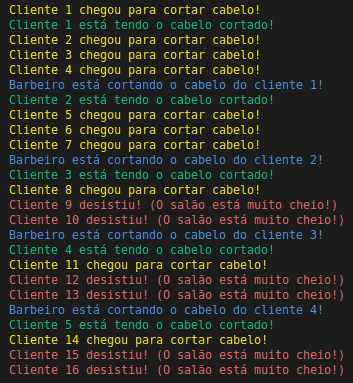
\includegraphics{imagens/out_barbeiro.png}
    \caption{Saída no terminal para o código barbeiro.c}
    \label{fig:out_barbeiro.c}
\end{figure}

A \textbf{Figura~\ref{fig:out_barbeiro.c}} mostra a saída no terminal pela execução do código \ovalbox{barbeiro.c}. É possível notar a chegada do primeiro cliente (1), que por ser o primeiro, obtém acesso imediato ao barbeiro, ainda disponível. Logo após, chegam mais clientes, que entram em espera pelo acesso ao corte de cabelo. O barbeiro, quando ocupado, imprime na tela que está cortando o cabelo de determinado cliente. No que se segue, chegam mais clientes, que entram em espera, se tiverem lugares. Se um cliente chega e não tem mais lugares, ele desiste e vai embora. 

Observe que, conforme o fluxo do código, mantemos o barbeiro ocupado 100\% do tempo, indicando sempre qual dos clientes ele está atendendo.

\subsection{Análise}
\subsubsection{Da solução implementada}

A solução implementada não apresenta soluções extraordinárias para o problema, mas faz bom uso dos semáforos como recurso controlador para o barbeiro e o número de clientes na barbearia. 

É interessante o uso do semáfor \ovalbox{cliente} não só como controle, mas também como contador de clientes e indicador para o barbeiro saber se deve trabalhar ou permanecer em espera, usado na função \ovalbox{barbeiro()}.

\subsection{De possíveis melhorias}

A solução apresentada pelo código \ovalbox{barbeiro.c} aé suficiente para atender aos requisitos impostos no início do capítulo. Porém, podemos apontar melhorias a serem implementadas para melhor análise e estudo do problema:
\begin{enumerate}
    \item Pelo que é visto no código, depois de algumas iterações, o salão permanece saturado, e o barbeiro nunca para de trabalhar.;
    \item É possível aumentar o intervalo de tempo entre a chegada de novos clientes, para denotar certa aleatoriedade e implementação de possíveis novos fenômenos;
    \item Novos comportamentos podem ser adicionados às entidades do códigos para aumentar a complexidade.
\end{enumerate}

\section{Capturas da IDE mostando o código}
Nesta seção serão apresentadas capturas da tela da IDE mostrando os códigos apresentados acima, que se encontram, também disponíveis no
\href{https://github.com/jvictorferreira3301/Sistemas_Operacionais}{nosso repositório da disciplina}.

Por conta da extensão do código, as capturas foram dividas em figuras diferentes, como segue:

\begin{figure}[h]
    \centering
    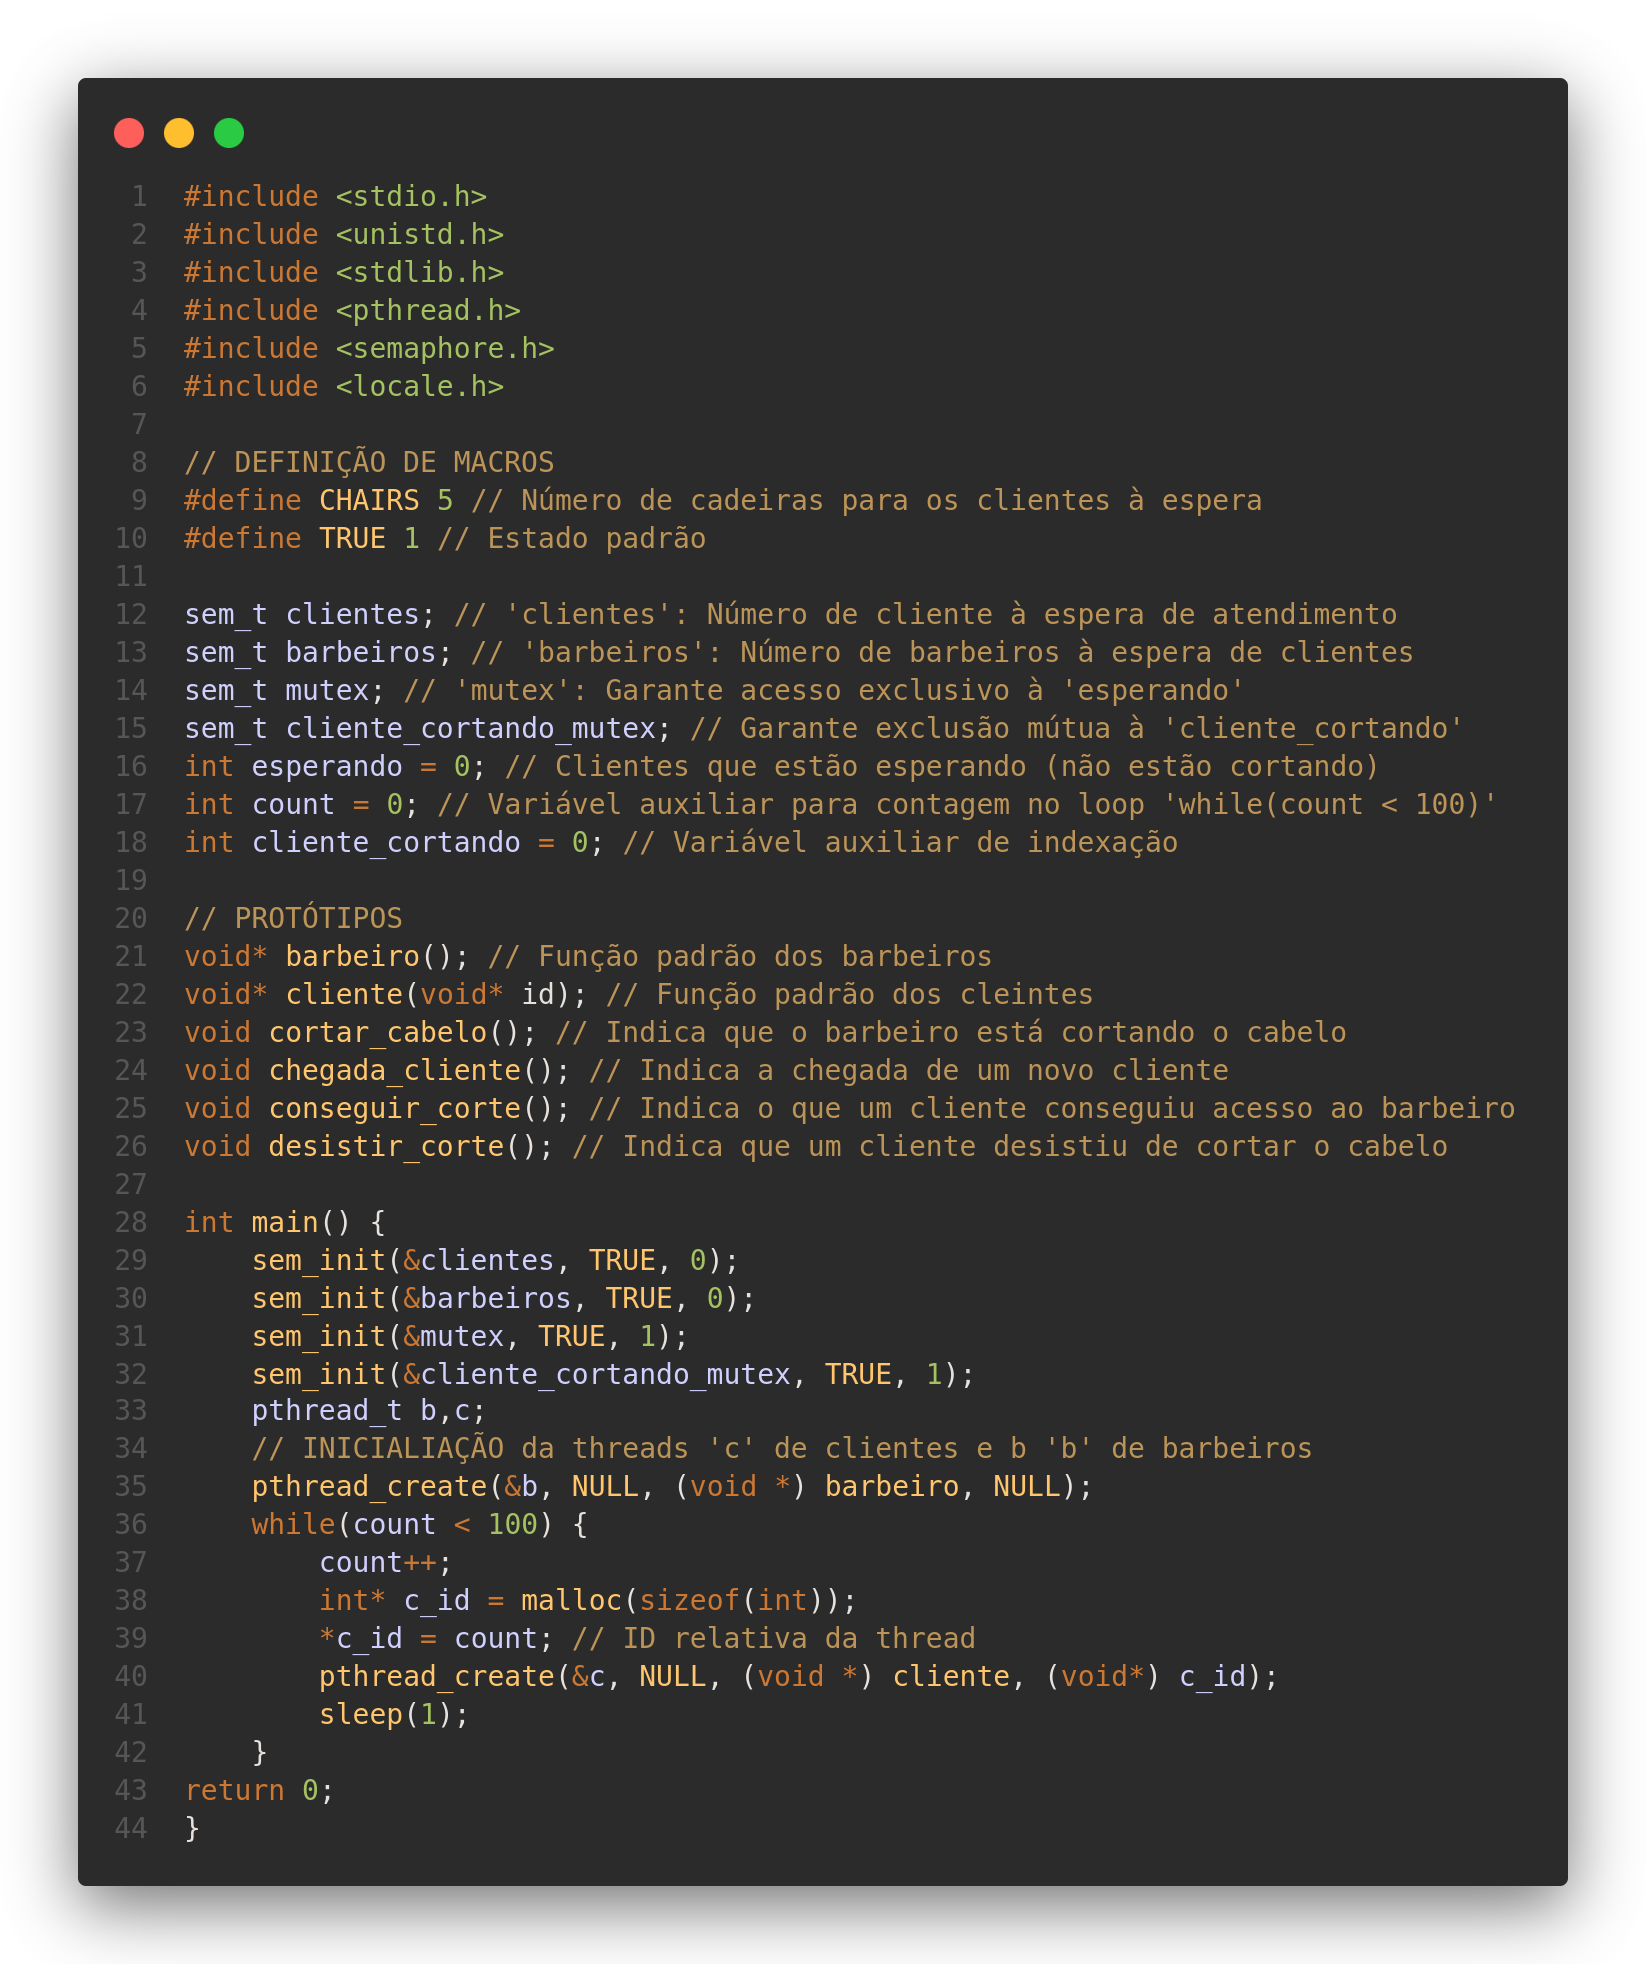
\includegraphics[width=1.0\textwidth]{imagens/barbeiro_1.png}
    \caption{O Barbeiro Dorminhoco: Código em C - Parte I}
    \label{fig:barbeiro_1}
\end{figure}

\begin{figure}[h]
    \centering
    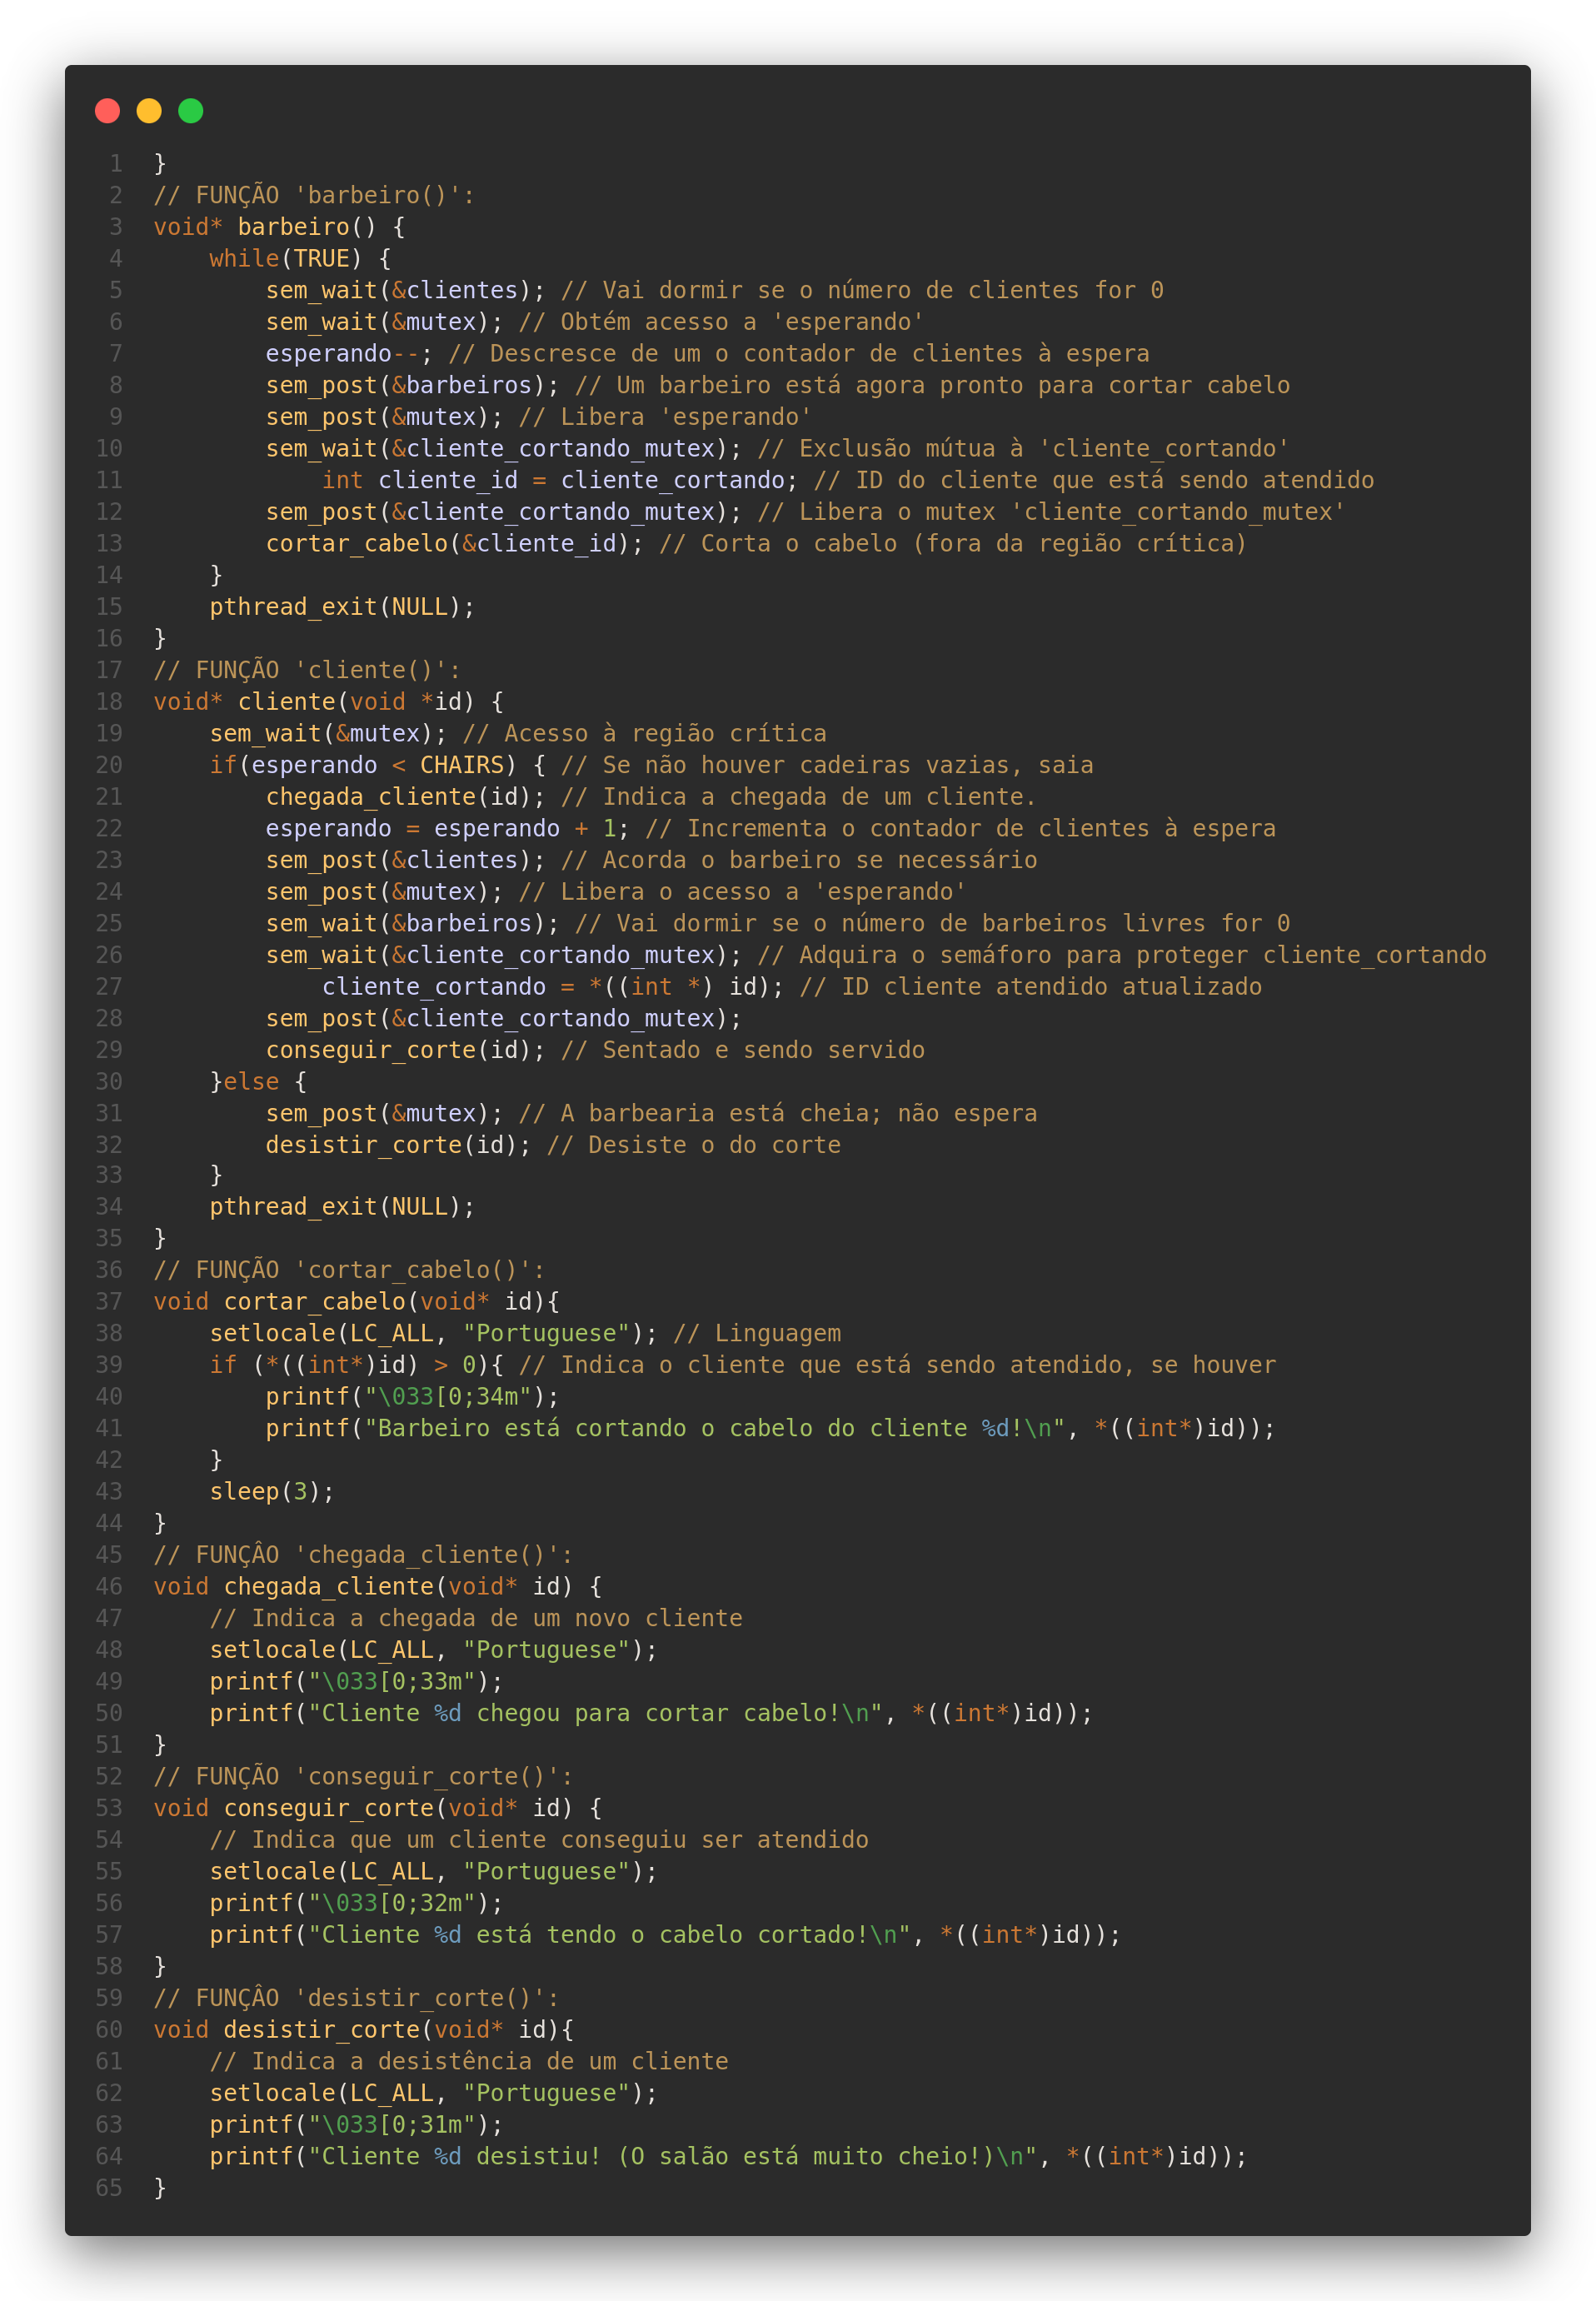
\includegraphics[width=1.0\textwidth]{imagens/barbeiro_3.png}
    \caption{O Barbeiro Dorminhoco: Código em C - Parte III}
    \label{fig:barbeiro_3}
\end{figure}

\clearpage
\section{Conclusão}

O Problema do Barbeiro Dorminhoco é um clássico problema em sistemas operacionais e proporciona boa visualização e entendimento de resoluções de situações em sincronização de tarefas. A solução empregada é eficiente em coordenar as threads criadas no código para se comportarem de maneira saudável durante o fluxo de execução, fazendo uso de semáforos para controlar o número de clientes e as ações do barbeiro. Por meio da saída no terminal, é possível ver como as threads se comportam concomitantemente, imprimindo as ações de acordo com o esperado.

\chapter{Conclusão}

Neste trabalho analisamos alguns dos problemas clássicos da literatura de sistemas operacionais. Por meio deles, foi possívei praticar o estudo do uso de semáforos e mutexes com objetivo de coordenar tarefas e sincronizar o acesso a regiões críticas.

Resolvendo o Problema do Leitor x Consumidor, observamos uma situação onde tarefas compartilham uma área de memória comum, e utilizamos semáforos e mutexes para coordenar o acesso exclusivo à essa área entre leitores e escritores, que desejam atuar sobre ela.

Solucionando o Problema do Jantar dos Filósofos, analisamos uma situação clara de prevenção de deadlock, onde tarefas concorrem ao acesso exclusivo a recursos compartilhados limitados. Fizemos uso de semáforos e mutexes para controlar o acesso a esses recursos e, por meio deles, garantimos a execução concomitante entre threads filósofos. 

Distrinchando o Problema do Produtor x Consumidor, discutimos como tarefas mutualmente dependentes podem ser coordenadas para manterem seus fluxos de execução sem entrarem em estados de inanição. Fizemos uso de semáforos e mutexes para mantero controle do estado do buffer do canal comparilhado entre produtores e consumidores, permitindo que ambos atuem concomitantemente.

Desvendando o Problema do Barbeiro Dorminhoco, percebemos como situações de espera com vagas limitadas podem ser trabalhadas. Fizemos uso de semáforos e mutexes para ter ciência do número de vagas de espera disponíveis, mantendo controle da lotação, bem como do estado de um fator ativo, no caso o barbeiro.

Por fim, foi possível o estudo, por meio dos problemas clássicos da literatura, de diferentes tópicos em comunicação inter-processos. Propusemos soluções para esses problemas, agregando conhecimento ao estudo de aplicações de semáforos, mutexes, processos e threads, objetos de estudo importantes para a compreensão e entendimento de diversos tópicos em sistemas operacionais.

\postextual

\bibliography{bibliografia}

\cite{tanenbaum2010sistemas}

\end{document}


